%%%%%%%%%%%%%%%%%%%%%%%%%%%%%%%%%%%%%%%%%%%%%%%%%%%%%%%%%%%%%%%%%%%%%%%%%%%%%%%%%%
%%																				%%
%% File name: 		T3X00.tex													%%
%% Project name:	Hochleistungsantenne										%%
%% Type of work:	T3X00 project work											%%
%% Author:			Sarah Brückner, Maximilian Stiefel, Hannes Bohnengel		%%
%% Date:			01st May 2016  												%%
%% University:		DHBW Ravensburg Campus Friedrichshafen						%%
%% Comments:		Created in gedit with tab width = 4							%%
%%																				%%
%%%%%%%%%%%%%%%%%%%%%%%%%%%%%%%%%%%%%%%%%%%%%%%%%%%%%%%%%%%%%%%%%%%%%%%%%%%%%%%%%%

%---- Define document class  -----------------------------------------------------

\documentclass[12pt]{report} % titlepage

%---- Define style ---------------------------------------------------------------

\usepackage{my_report}

%---- Include dynamic data -------------------------------------------------------

%%%%%%%%%%%%%%%%%%%%%%%%%%%%%%%%%%%%%%%%%%%%%%%%%%%%%%%%%%%%%%%%%%%%%%%%%%%%%%%%%%
%%																				%%
%% File name: 		data.tex													%%
%% Project name:	Hochleistungsantenne										%%
%% Type of work:	T3X00 project work											%%
%% Author:			Sarah Brückner, Maximilian Stiefel, Hannes Bohnengel		%%
%% Date:			01st May 2016												%%
%% University:		DHBW Ravensburg Campus Friedrichshafen						%%
%% Comments:		Created in gedit with tab width = 4							%%
%%																				%%
%%%%%%%%%%%%%%%%%%%%%%%%%%%%%%%%%%%%%%%%%%%%%%%%%%%%%%%%%%%%%%%%%%%%%%%%%%%%%%%%%%

\newcommand{\mytitle}{Inbetriebnahme einer freien Software zur Satellitenbahnvorhersage und Ansteuerung einer Hochleistungsantenne}
\newcommand{\myauthora}{Sarah Brückner}
\newcommand{\myauthorb}{Maximilian Stiefel}
\newcommand{\myauthorc}{Hannes Bohnengel}
\newcommand{\mytutor}{Dipl.-Ing. (DH) Hardy Lau}
\newcommand{\mytypeofwork}{Studienarbeit}
\newcommand{\myduedate}{15. Juli 2016}
\newcommand{\myuniversity}{DHBW Ravensburg}
\newcommand{\myuniversitycampus}{Friedrichshafen}
\newcommand{\mycourse}{Elektrotechnik, Nachrichten- und Kommunikationstechnik}
\newcommand{\myplace}{Friedrichshafen}
\newcommand{\mykeywords}{Antennennachführung, CubeSat, Java, Keppler}


%---- Hyperref -------------------------------------------------------------------

\usepackage{hyperref} 
\hypersetup{
	plainpages=false,
	unicode=false,
	pdftoolbar=true,
	pdfmenubar=true,
	pdffitwindow=false,
	pdfstartview={FitH},
	pdftitle={\mytitle},
	pdfauthor={\myauthora,\space\myauthorb,\space\myauthorc},
	pdfsubject={\mytypeofwork},
	pdfcreator={\mytutor},
	pdfproducer={\LaTeX},
	pdfkeywords={\mykeywords},
	pdfnewwindow=true,
	pdfborder={0 0 0},
	colorlinks=false,
	linkcolor=black,
	citecolor=black,
	filecolor=black,
	urlcolor=cyan
}

%---- Begin of document ----------------------------------------------------------

\begin{document}

%---- Title page -----------------------------------------------------------------

%%%%%%%%%%%%%%%%%%%%%%%%%%%%%%%%%%%%%%%%%%%%%%%%%%%%%%%%%%%%%%%%%%%%%%%%%%%%%%%%%%
%%																				%%
%% File name: 		titlepage.tex												%%
%% Project name:	Hochleistungsantenne										%%
%% Type of work:	T3X00 project work											%%
%% Author:			Sarah Brückner, Maximilian Stiefel, Hannes Bohnengel		%%
%% Date:			29th April 2016												%%
%% University:		DHBW Ravensburg Campus Friedrichshafen						%%
%% Comments:		Created in gedit with tab width = 4							%%
%%																				%%
%%%%%%%%%%%%%%%%%%%%%%%%%%%%%%%%%%%%%%%%%%%%%%%%%%%%%%%%%%%%%%%%%%%%%%%%%%%%%%%%%%

\begin{titlepage}
% temporary margins only for titlepage
\newgeometry{lmargin={2cm},rmargin={2cm},tmargin={1cm},bmargin={2cm}}

%---------------------- Figures --------------------------------------------------

\begin{figure}
	%\raggedright
	\raggedleft
	
\includegraphics[width=0.4\textwidth]{dhbw}
\end{figure}

%---------------------- Text -----------------------------------------------------

\begin{center}
	\vspace*{0pt}
	\begin{LARGE}
		\textbf{\mytitle}\\
	\end{LARGE}
	\vspace*{4em}
	\textbf{\MakeUppercase{\mytypeofwork}\\über das dritte Studienjahr}\\
	\vspace*{2em}
	im Studiengang\\
	\mycourse\\
	\vspace*{2em}
	an der \myuniversity\\
	Campus \myuniversitycampus\\
	\vspace*{2em}
	von\\
	\vspace*{2em}
	\myauthora,\\\myauthorb\ und\\\myauthorc\\
	\vspace*{2em}
	\today\\
	\vspace*{3em}
	\vfill
%---------------------- Table ----------------------------------------------------
	
	\setlength{\tabcolsep}{24pt}	% change space between rows
	\begin{tabular}{ll}
		Bearbeitungszeitraum:&Oktober - Dezember 2015\\
		&April - Juni 2016\\
		%Matrikelnummern:&4167768\\
		%&1231235\\
		%&4564567\\
		Betreuer:&\mytutor\\
	\end{tabular}
	\setlength{\tabcolsep}{6pt}		% back to default
	\restoregeometry
\end{center}
\end{titlepage}
\clearpage


%---- Abstract -------------------------------------------------------------------

%%%%%%%%%%%%%%%%%%%%%%%%%%%%%%%%%%%%%%%%%%%%%%%%%%%%%%%%%%%%%%%%%%%%%%%%%%%%%%%%%%
%%																				%%
%% File name: 		abstract.tex												%%
%% Project name:	Hochleistungsantenne										%%
%% Type of work:	T3X00 project work											%%
%% Author:			Sarah Brückner, Maximilian Stiefel, Hannes Bohnengel		%%
%% Date:			11th July 2016												%%
%% University:		DHBW Ravensburg Campus Friedrichshafen						%%
%% Comments:		Created in gedit with tab width = 4							%%
%%																				%%
%%%%%%%%%%%%%%%%%%%%%%%%%%%%%%%%%%%%%%%%%%%%%%%%%%%%%%%%%%%%%%%%%%%%%%%%%%%%%%%%%%

\chapter*{Kurzfassung}
Diese Studienarbeit beschreibt die Inbetriebnahme einer freien Software zur Satellitenbahnvorhersage und Ansteuerung einer Hochleistungsantenne. 
Dies schließt die Nachführung der Antenne und damit die Steuerung von Rotoren mit ein. Die freie Software soll die bestehende Software 
SatPC32 ersetzen. SatPC32 ist eine proprietäre Software und dient der Bodenstation als Referenz. Da SatPC32 nicht mehr weiterentwickelt wird 
und es darüber hinaus keinen Support für diese Software gibt, wurde der alternative Weg, einer freien Software für die Bodenstation in 
Friedrichshafen, gewählt. Diese freie Software ist GPredict. GPredict ist quelloffen und beherrscht es mit Hilfe der \ac{TLE} die Satellitenposition 
vorherzusagen und diese auf einer grafischen Oberfläche anzuzeigen. Des Weiteren wird von GPerdict bzw. der darunter liegenden HamLib eine Vielzahl 
verschiedener Hardware-Einheiten zur Ausrichtung der Antenne und zur Kommunikation unterstützt. Eine Kommunikation mit Transpondern im Orbit 
aufzubauen ist somit durch GPredict realisierbar.
 
\vspace{3em}
\begin{Huge}
	\textbf{Abstract}
\end{Huge}
\vspace{1.5em}

Translation of ,,Kurzfassung'' comes here...

\clearpage


%---- Statement of Authentication ------------------------------------------------

%%%%%%%%%%%%%%%%%%%%%%%%%%%%%%%%%%%%%%%%%%%%%%%%%%%%%%%%%%%%%%%%%%%%%%%%%%%%%%%%%%
%%																				%%
%% File name: 		statement.tex												%%
%% Project name:	Hochleistungsantenne										%%
%% Type of work:	T3X00 project work											%%
%% Author:			Sarah Brückner, Maximilian Stiefel, Hannes Bohnengel		%%
%% Date:			29th April 2016											%%
%% University:		DHBW Ravensburg Campus Friedrichshafen						%%
%% Comments:		Created in gedit with tab width = 4							%%
%%																				%%
%%%%%%%%%%%%%%%%%%%%%%%%%%%%%%%%%%%%%%%%%%%%%%%%%%%%%%%%%%%%%%%%%%%%%%%%%%%%%%%%%%

\chapter*{Erklärung}
\pagenumbering{gobble} 		% suppress displaying the page number

gemäß Ziffer 1.1.13 der Anlage 1 zu §§ 3, 4 und 5  der Studien- und Prüfungsordnung für die Bachelorstudiengänge im Studienbereich Technik der Dualen Hochschule Baden-Württemberg vom 29.09.2015.\\[1em]
Wir versichern hiermit, dass wir unsere \mytypeofwork\ mit dem Thema:
\vspace{24pt}
\begin{large}
\begin{center}
	\textbf{\mytitle}
\end{center}
\end{large}
\vspace{24pt}
selbstständig verfasst und keine anderen als die angegebenen Quellen und Hilfsmittel benutzt haben. Wir versichern zudem, dass die eingereichte elektronische Fassung mit der gedruckten Fassung übereinstimmt.\\[2em]
\myplace, den \today\\[6em]
\begin{raggedright}
	\begin{tabular}[h]{p{7cm}}
		\cline{1-1}
		\myauthora\\
	\end{tabular}
\end{raggedright}\\[4em]

\begin{raggedright}
	\begin{tabular}[h]{p{7cm}}
		\cline{1-1}
		\myauthorb\\
	\end{tabular}
\end{raggedright}\\[4em]

\begin{raggedright}
	\begin{tabular}[h]{p{7cm}}
		\cline{1-1}
		\myauthorc\\
	\end{tabular}
\end{raggedright}

\clearpage


%---- Table of contents ----------------------------------------------------------

\tableofcontents
\clearpage

%---- vvv ROMAN PAGE NUMBERING vvv -----------------------------------------------

\pagenumbering{Roman}

%---- Physical Quantities --------------------------------------------------------

%%%%%%%%%%%%%%%%%%%%%%%%%%%%%%%%%%%%%%%%%%%%%%%%%%%%%%%%%%%%%%%%%%%%%%%%%%%%%%%%%%
%%																				%%
%% File name: 		physical_quantities.tex										%%
%% Project name:	Hochleistungsantenne										%%
%% Type of work:	T3X00 project work											%%
%% Author:			Sarah Brückner, Maximilian Stiefel, Hannes Bohnengel		%%
%% Date:			25th April 2016	     										%%
%% University:		DHBW Ravensburg Campus Friedrichshafen						%%
%% Comments:		Created in gedit with tab width = 4							%%
%%																				%%
%%%%%%%%%%%%%%%%%%%%%%%%%%%%%%%%%%%%%%%%%%%%%%%%%%%%%%%%%%%%%%%%%%%%%%%%%%%%%%%%%%

\chapter*{Formelgrößen und Einheiten}
% To add "Formelgrößen und Einheiten" to toc
\addcontentsline{toc}{chapter}{Formelgrößen und Einheiten}
\begin{tabularx}{\textwidth}{|l|l|l|X|}
	\hline
	\textbf{Formelzeichen} 	& \textbf{Einheit}			&\textbf{Abkürzung}     		& \textbf{Physikalische Größe} \\ \hline
	\ensuremath{r}         	& Meter 	 				&\ensuremath{m}					& Länge\hspace{10cm}  	\\   
	\ensuremath{v=\dot{r}}  & Meter pro Sekunde		 	&\ensuremath{\frac{m}{s}}		& Geschwindigkeit\hspace{10cm}  	\\   
	\ensuremath{a=\dot{v}=\ddot{r}}         			& Meter pro Quadratsekunde&\ensuremath{\frac{m}{s^2}}& Beschleunigung\hspace{10cm}  	\\
	\ensuremath{A}         	& Quadratmeter		 	&\ensuremath{m^2}		&Fläche \hspace{10cm}  	\\
	\ensuremath{M}         	& Kilogramm		 			&\ensuremath{kg}				& Masse\hspace{10cm}  	\\
	\hline		
\end{tabularx}
\clearpage


%---- Abbreviations --------------------------------------------------------------

%%%%%%%%%%%%%%%%%%%%%%%%%%%%%%%%%%%%%%%%%%%%%%%%%%%%%%%%%%%%%%%%%%%%%%%%%%%%%%%%%%
%%																				%%
%% File name: 		abbreviations.tex											%%
%% Project name:	Hochleistungsantenne										%%
%% Type of work:	T3X00 project work											%%
%% Author:			Sarah Brückner, Maximilian Stiefel, Hannes Bohnengel		%%
%% Date:			21th May 2016												%%
%% University:		DHBW Ravensburg Campus Friedrichshafen						%%
%% Comments:		Created in gedit with tab width = 4							%%
%%																				%%
%%%%%%%%%%%%%%%%%%%%%%%%%%%%%%%%%%%%%%%%%%%%%%%%%%%%%%%%%%%%%%%%%%%%%%%%%%%%%%%%%%

\chapter*{Abkürzungen}
% To add "Abkürzungen" to toc
\addcontentsline{toc}{chapter}{Abkürzungen}

\begin{acronym}[GPL123]	% put the longest abbreviation in brackets to adjust indentation
%\setlength{\itemsep}{0.5em}
	\acro{API}{Application Programming Interface}	
	\acro{AOS}{Acquisiton of Signal}
	\acro{BE} {Backend}
	\acro{CAT}{Computer Aided Tuning}
	\acro{LOS}{Loss of Signal}
	\acro{GPL}{General Public License}
	\acro{SSP}{Sub-Satellite Point}
	\acro{CW}{Continious Wave}
	\acro{SGP4}{„Simplified General Pertubations Model No. 4“ }
	\acro{SDP4}{„Simplified Deep Space Pertubations Model No. 4“ }
	\acro{NORAD}{„North American Aerospace Defense Command“}
	\acro{TLE}{„Two-line Elements“}
\end{acronym}
\clearpage


%---- vvv ARABIC PAGE NUMBERING vvv ----------------------------------------------

\setcounter{romanPagenumber}{\value{page}}
\pagenumbering{arabic}
\setcounter{page}{1}

%---- Introduction ---------------------------------------------------------------

%%%%%%%%%%%%%%%%%%%%%%%%%%%%%%%%%%%%%%%%%%%%%%%%%%%%%%%%%%%%%%%%%%%%%%%%%%%%%%%%%%
%%																				%%
%% File name: 		introduction.tex											%%
%% Project name:	Hochleistungsantenne										%%
%% Type of work:	T3X00 project work											%%
%% Author:			Sarah Brückner, Maximilian Stiefel, Hannes Bohnengel		%%
%% Date:			07th June 2016												%%
%% University:		DHBW Ravensburg Campus Friedrichshafen						%%
%% Comments:		Created in gedit with tab width = 4							%%
%%																				%%
%%%%%%%%%%%%%%%%%%%%%%%%%%%%%%%%%%%%%%%%%%%%%%%%%%%%%%%%%%%%%%%%%%%%%%%%%%%%%%%%%%

\chapter{Einleitung}
In der Vergangenheit wurden teure Satelliten nur zu Forschungs-- und Verteidigungszwecken entwickelt und gebaut. Heutzutage nimmt der 
Geschäftsanteil mit kommerziellen Satelliten stetig zu. Möchte der Fussball--Fan ein Europameisterschaftsspiel in Echtzeit verfolgen können oder der 
Reisende sich zu seinem Ziel navigieren lassen, so sind Satellitensysteme unverzichtbar.
\newpar
Eine entscheidende Rolle bei der Satellitenforschung haben die 
Amateurfunksatelliten 
gespielt. Neue Techniken konnten ohne ein kommerzielles Geschäft oder eine wissenschaftliche bzw. militärische Mission zu gefährden mit 
Amateurfunksatelliten getestet werden. Die ständige Beobachtung der Satelliten wurde durch die 
Vielzahl der Amateurfunker weltweit sichergestellt. 
\newpar
Um Satelliten in der Nachrichtentechnik nutzen zu können, wird eine Bodenstation benötigt. Mit entsprechender Hard- und 
Software können Satelliten verfolgt werden. Auch eine Kommunikation über und mit Objekten im Orbit ist durch ein entsprechendes Equipment möglich. 
\newpar
Diese Studienarbeit beschreibt die Inbetriebnahme einer freien Software 
zur Satellitenbahnvorhersage und Ansteuerung einer Hochleistungsantenne. Dies schließt die Nachführung der Antenne und damit die Steuerung von 
Rotoren mit ein. Die freie Software soll die bestehende Software 
SatPC32 ersetzen. SatPC32 ist eine proprietäre Software und dient der Bodenstation als Referenz. Da SatPC32 nicht mehr weiterentwickelt wird 
und es darüber hinaus keinen Support für diese Software gibt, wurde der alternative Weg, einer freien Software für die Bodenstation in 
Friedrichshafen, gewählt. Diese freie Software ist GPredict. GPredict ist quelloffen und beherrscht es mit Hilfe der \ac{TLE} die Satellitenposition 
vorherzusagen. Des Weiteren wird von GPerdict bzw. der darunter liegenden HamLib eine Vielzahl verschiedener Hardware-Einheiten zur Ausrichtung der 
Antenne und zur Kommunikation unterstützt. Die Ausgabe der Satellitenposition auf einer grafischen Oberfläche beherrscht GPredict problemlos. Eine 
Kommuniktaion mit Transpondern im Orbit aufzubauen ist mit GPredict kinderleicht.
\newpar
Diese Studienarbeit beschreibt GPredict und soll dem Leser einen 
leichten Einstieg in die Bedienung dieser Software ermöglichen. Außerdem beleuchtet diese Arbeit den physikalischen Hintergrund der 
Satellitenbahn-Vorhersage und damit einhergehend die Ursache der Dopplerverschiebung der Mittenfrequenz bei der Kommunikation mit einem Satelliten. 
Ein weiterer inhaltlicher Grundpfeiler dieser Studienarbeit ist die Dokumentation des gesamten Projektprozess. 
%  In der heutigen Gesellschaft ... Satelliten kaum mehr wegzudenken ... mobile Kommunikation, Navigation, Forschung, Satellitenfernsehen ...\\
%  Bei der Entwicklung und dem Test der Kommunikation zwischen Erde und Satellit haben Amateurfunksatelliten und Amateurfunkbodenstationen eine entscheidende Rolle gespielt (Quelle Amsat-Website)...\\
%  An der Dualen Hochschule Baden-Württemberg am Campus Friedrichshafen soll eine solche Bodenstation errichtet werden.\\
%  Die Software SatPC32 soll ersetzt werden und dient dabei als Referenz.

\clearpage


%---- Main part ------------------------------------------------------------------

% Projektmanagmenet
%%%%%%%%%%%%%%%%%%%%%%%%%%%%%%%%%%%%%%%%%%%%%%%%%%%%%%%%%%%%%%%%%%%%%%%%%%%%%%%%%%
%%																				%%
%% File name: 		00sarah.tex													%%
%% Project name:	Hochleistungsantenne										%%
%% Type of work:	T3X00 project work											%%
%% Author:			Sarah Brückner, Maximilian Stiefel, Hannes Bohnengel		%%
%% Date:			27th Arpil 2016												%%
%% University:		DHBW Ravensburg Campus Friedrichshafen						%%
%% Comments:		Created in gedit with tab width = 4							%%
%%																				%%
%%%%%%%%%%%%%%%%%%%%%%%%%%%%%%%%%%%%%%%%%%%%%%%%%%%%%%%%%%%%%%%%%%%%%%%%%%%%%%%%%%
%\cite{kauffels}\newpar

\chapter{Projektmanagement}
Schon Thomas Carlyle (1795–1881) erkannte die Wichtigkeit von strukturierten und organisiertem Vorgehen als er sagte:\newpar
``Unsere Hauptaufgabe ist nicht, zu erkennen, was unklar in weiter Entfernung liegt, sondern zu tun, was klar vor uns liegt''.\newpar
In einem Projekt ist das strukturierte und ogranisierte Vorgehen der klare Weg zu einem erfolgreichem Ziel. Daher wird sich in dieser Arbeit
dem Projektmanagement bedient um die Antennennachführung für Satelliten in die richtige Richtung zu lotzen. Dabei lehnt sich das Management an 
das bekannte V-Modell, welche den Abflauf von Software-, als auch von Hardwareentwicklungsprozessen beschreibt. Dieses Modell soll einem Projekt 
die Richtung weisen, jedoch werden die einzelnen Schritte vom Projektmanager selbst definiert. Ein Vorgehensmodell wie dieses legt folgende
Prozesse fest:
\begin{itemize}
 \item die Aktivitäten die durchzuführen sind,
 \item die Reihenfolge des Arbeitsablaufes,
 \item die Definition von Ergebnissen,
 \item die Fertigstellungskriterien,
 \item die Ressourcen die vorhanden sind
 \item und die anzuwendenden Standards/Werkzeuge.
\end{itemize}
\begin{figure}[h]
 \centering
 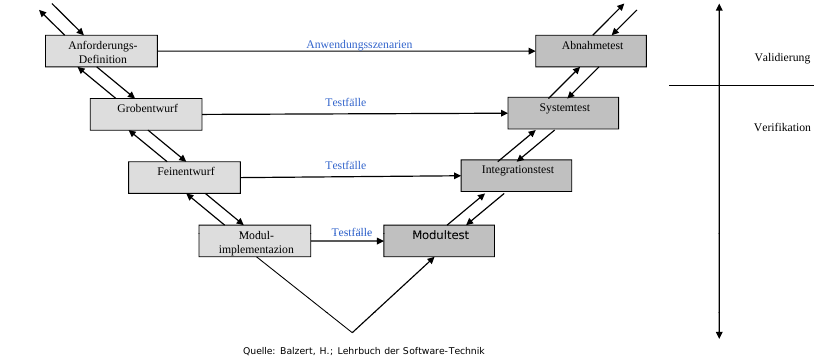
\includegraphics[width=0.8\linewidth]{./images/vmodell}
 \caption{V-Modell, Quelle: Universität Leipzig, Softwaretechnik}
 \label{fig:vmodell}
\end{figure}
Eine wichtige Rolle spielt die Qualitätssicherung, die das V-Modell sicher stellt. In diesem Modell sind die Verifikation und die Validation ein 
fester Bestandteil. Verifikation bedeutet, die Sicherstellung dass das entwickelte Produkt mit den Spezifikationen übereinstimmt.
Die Validation ist die Eignung des Produkts bezogen auf seinen Einsatzzweck. Durch die Sicherstellung beider Qualitätsmerkmale wird das Projekt 
erfolgreich zu seinem Ziel, die Antnennennachführung für Satelliten, geführt.Aus diesem Grund ist das V-Modell die richtie Vorangehensweise für 
dieses Projekt.\newpar

\section{Zeitplan}
\section{Anforderungsdefinition}
\section{Arbeitspakete}






% Theorie
%%%%%%%%%%%%%%%%%%%%%%%%%%%%%%%%%%%%%%%%%%%%%%%%%%%%%%%%%%%%%%%%%%%%%%%%%%%%%%%%%%
%%																				%%
%% File name: 		10max.tex													%%
%% Project name:	Hochleistungsantenne										%%
%% Type of work:	T3X00 project work											%%
%% Author:			Sarah Brückner, Maximilian Stiefel, Hannes Bohnengel		%%
%% Date:			27th Arpil 2016												%%
%% University:		DHBW Ravensburg Campus Friedrichshafen						%%
%% Comments:		Created in gedit with tab width = 4							%%
%%																				%%
%%%%%%%%%%%%%%%%%%%%%%%%%%%%%%%%%%%%%%%%%%%%%%%%%%%%%%%%%%%%%%%%%%%%%%%%%%%%%%%%%%

\chapter{Hintergründe}

\section{Bahnmechanik}
\subsection{Die Keplerschen Gesetze}
\label{subsec:kepler}
Seit der Antike galt die Erklärung der Bewegung der Planeten und die Vorhersage dieser als eine große Herausforderung. Theorien von Ptolemaios mit seinem geozentrischen Weltbild und Kopernikus mit seinem heliozentrischen Weltbild führten bereits im 16. Jahrhundert zu brauchbaren Modellen zur Vorhersage der Planetenbewegungen. Diese Modelle unterlagen jedoch Ungenauigkeiten, „die in mit Instrumenten des 16. Jahrhunderts bereits messbaren Breichen lagen“ (siehe S. 20 in \cite{Raumflugm}). 
%%%%%%%%%%%%%%%%%%%%%%%%%%%%%%%%%%%%%%%%%%%%%%%%%%%%%%%%%%%%%%%%%%%%%%%%%%%%%%%%%%%%%%%%%%%%%%
\begin{figure}[h]                                                                           %%
	\centering                                                                            	%%
	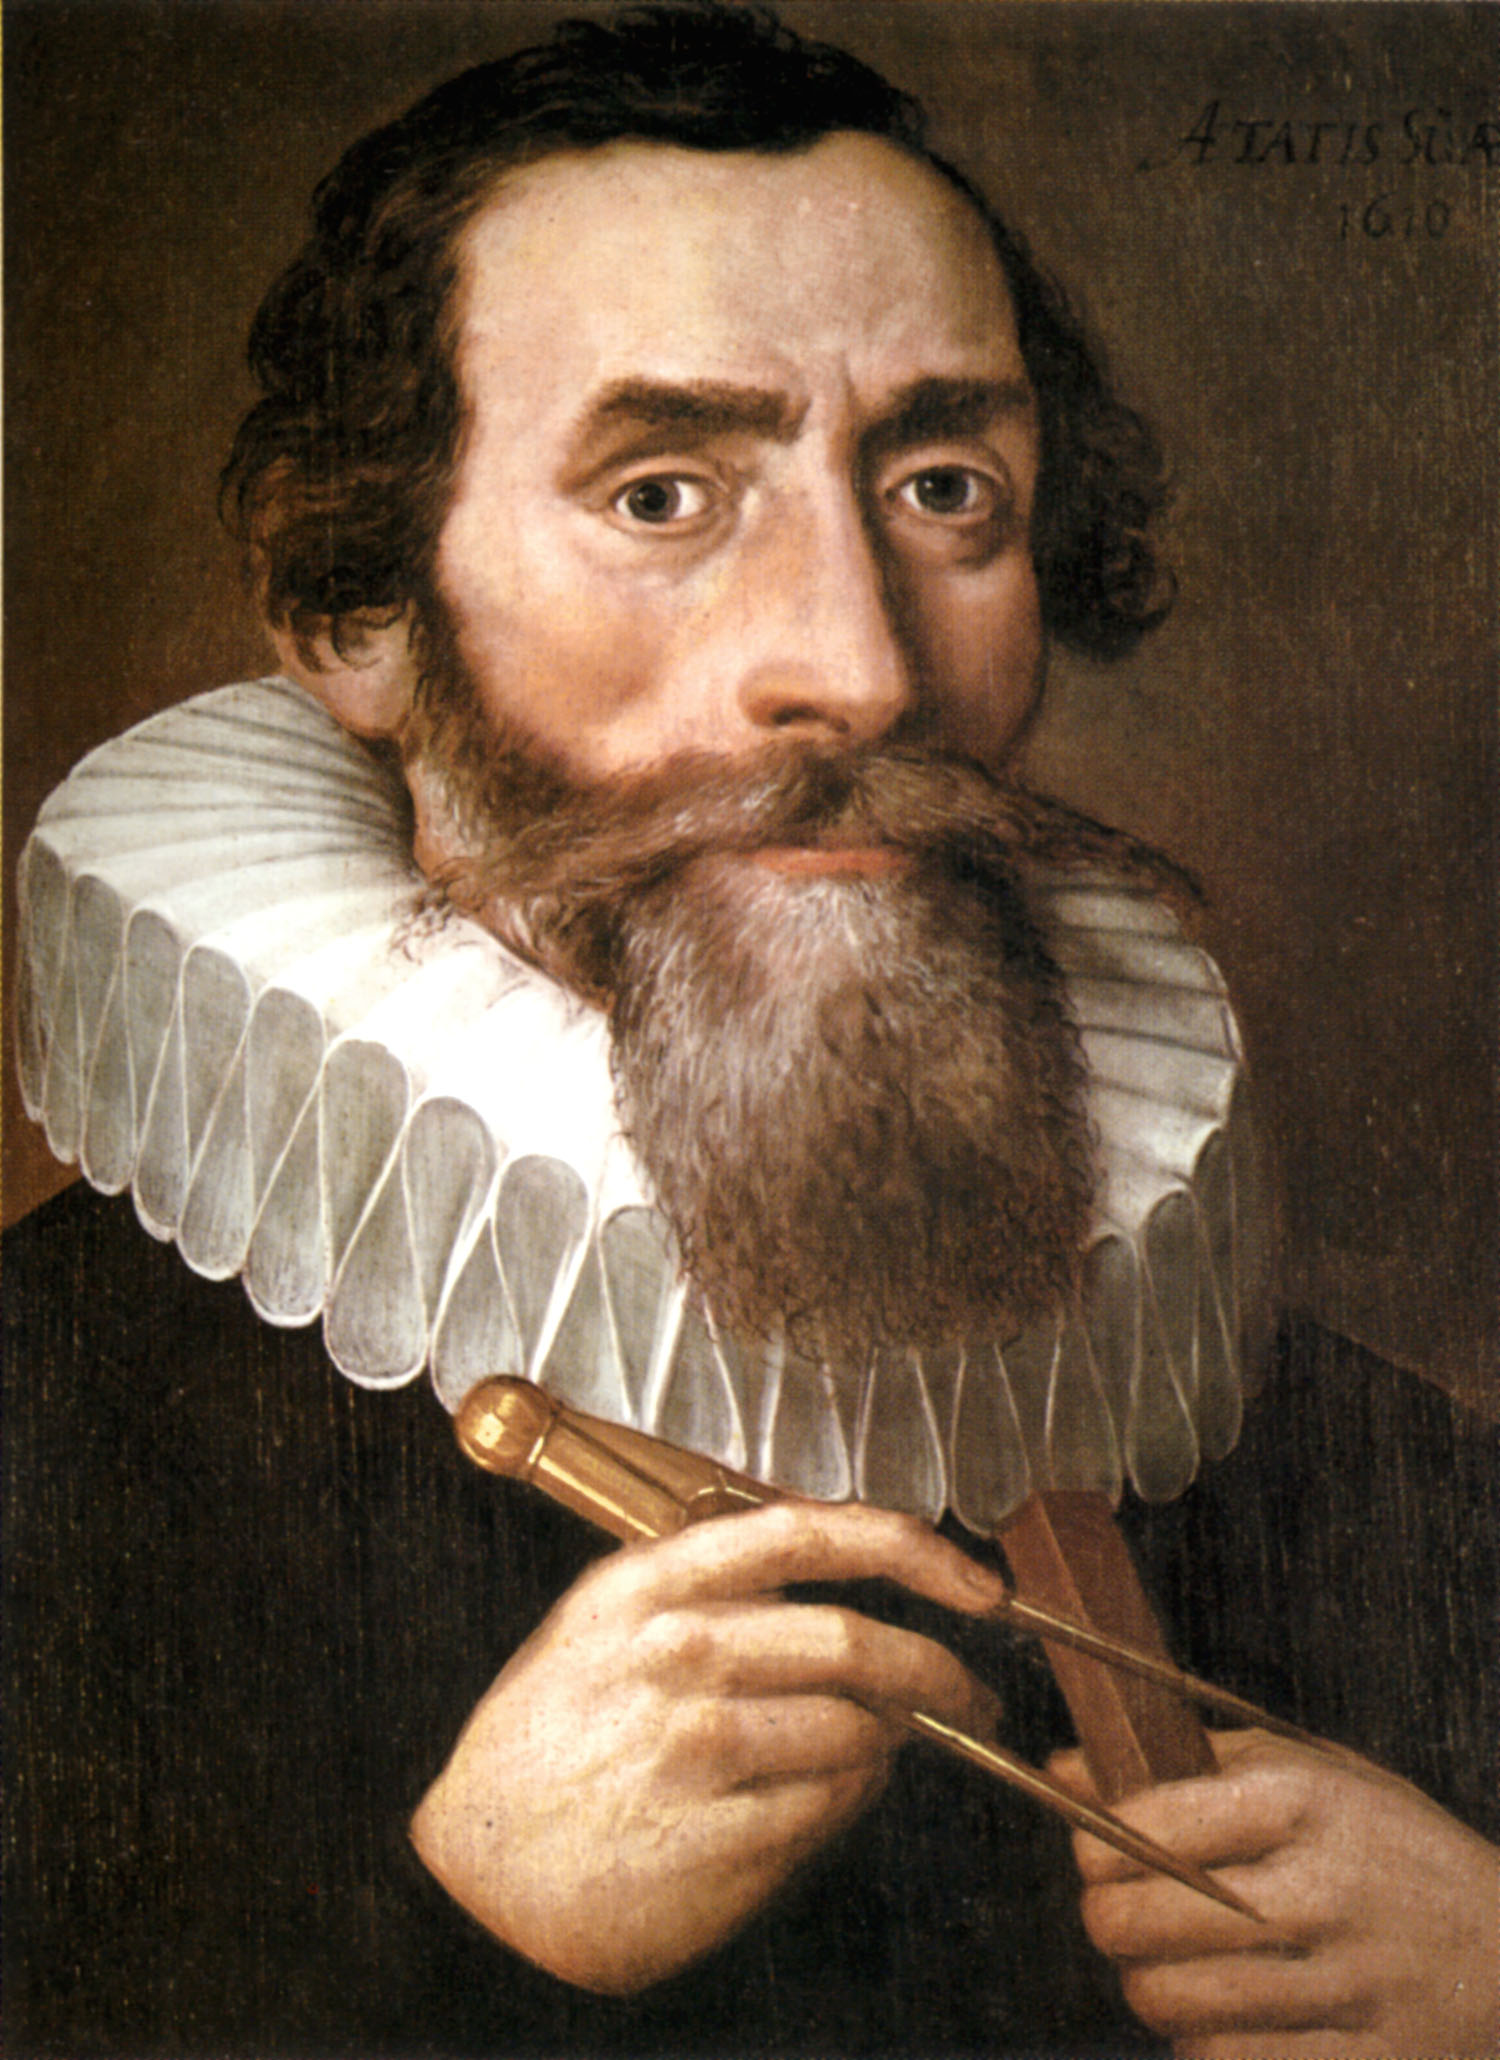
\includegraphics[width=0.3\textwidth]{./images/kepler.jpg}                              %%
	\caption[Bahnelemente]{Johannes Kepler (1571-1630), Quelle: \cite{Wiki:Kepler}}         %%
	\label{fig:kepler}                                                                %%
\end{figure}                                                                              	%%
%%%%%%%%%%%%%%%%%%%%%%%%%%%%%%%%%%%%%%%%%%%%%%%%%%%%%%%%%%%%%%%%%%%%%%%%%%%%%%%%%%%%%%%%%%%%%% 
Der mathematische Aufwand hinter diesen Modellen war enorm. Selbst das kopernikanische Weltbild, dass einige Vereinfachnugen mit sich brachte, bediente sich der Überlagerung einer Vielzahl von Kreisbwegungen, um das Verhalten der Planeten zu erklären. Resignierend zog sich zu der Zeit die katholische Kirsche und mit ihr viele Gelehrte auf den Standpunkt zurück, dass „die Frage, welche der Theorien die korrekte sei, [...] schlicht unbeantwortbar“ wäre (siehe S. 21 in \cite{Raumflugm}). 
\newpar
Ein deutscher Mathematiker und Astronom, Johannes Kepler, war hier anderer Auffassung. Er war überzeugter Kopernikaniker und stand im Dienste des Kaisers Rudolph II. Schließlich gelang es ihm aus seinen Beobachtungen drei einfache Gesetze herzuleiten. Seine Gesetze führten zu Vorhersagen der Planetenbewegungen nie da gewesener Präzision, welche er seinem Dienstherr widmend in den Rudolphinischen Tabellen niederschrieb. Steiner und Schlagerl schreiben in Ihrem Buch „Raumflugmechanik“, dass ohne die Vorarbeit Keplers keine Weltraumtechnik je existiert hätte (vgl. S. 21 in \cite{Raumflugm}). Die drei Gesetze lauten:
\begin{enumerate}
	\item Keplersches Gesetz: Die Planeten umlaufen die Sonne auf elliptischen Bahnen. In einem der Brennpunkte dieser Ellipsen befindet sich die Sonne. 
	\item Keplersches Gesetz: Die Linie von der Sonne zu einem Planeten überstreicht in gleichen Zeiten gleiche Flächen.
	\item Keplersches Gesetz: Die Quadrate der Umlaufzeiten zweier Planeten verhalten sich zueinander so wie die Kuben der großen Halbachsen ihrer Bahnellipsen. 
\end{enumerate}   
Kepler starb 1630 und damit 12 Jahre vor Isaac Newtons (1642-1726) Geburt. Mit seinen Werken hinterließ Kepler Newton alles, um das Gravitationsgesetz später herleiten zu können. 
\subsubsection{Das erste Keplersche Gesetz}
Durch die Annahme Planeten bewegen sich auf Ellipsen anstatt auf Kreisen, brach Kepler ein tausende Jahre altes Paradigma. Das mit der Ellipse war allerdings nicht seine Idee. Bereits im 11. Jahrhundert nahm ein arabischer Gelehrter namens Al-Zarkali (1029-1087) eine elliptische Bahn an, um die unregelmäßige Bewegung des Merkurs erklären zu können. Kepler kannte diese Idee durch die Lehren des Mathematikers und Astronomen Peuerbach (1423-1461), welcher die Ellipsen-Theorie im Abendland verbreitete.  
\newpar
Zunächst soll die Ellipse an sich betrachtet werden. Die einfachste Möglichkeit eine Ellipse zu konstruieren besteht darin zwei Nägel in einer Holzplatte mit einem Stück Schnur mit einer Schlaufe zu verbinden. Das Stück Schnur muss länger sein als der Abstand zwischen beiden Nägeln. Nimmt man nun einen Bleistift und drückt ihn in der Schlaufe gegen die Schnur, kann man die beiden Nägel mit Kontakt der Bleistiftspitze zum Holzbrett umrunden. Hält man die Schnur konstant auf Spannung, so ergibt sich eine Ellipse. Darüber hinaus muss der Punkt auf welchem die Schlaufe am Bleistift anliegt höher sein, als der Abschluss der Nagelköpfe. Im übertragenden Sinne beschreibt die folgende Mengendefinition dieses Experiment mit Bezug zu Abbildung \ref{fig:ellipse}. 
\begin{equation}
E = \{P | \overline{F_{1}P} + \overline{F_{2}P} = 2a = konstant\}
\end{equation}
\ensuremath{F_{1}} und \ensuremath{F_{2}} heißen Brennpunkte der Ellipse. \ensuremath{M} ist der Mittelpunkt der Ellipse. \ensuremath{S_{1}} und \ensuremath{S_{2}} sind die Haupt-, \ensuremath{S_{3}} und \ensuremath{S_{4}} die Nebenscheitel.      
%%%%%%%%%%%%%%%%%%%%%%%%%%%%%%%%%%%%%%%%%%%%%%%%%%%%%%%%%%%%%%%%%%%%%%%%%%%%%%%%%%%%%%%%%%%%%%
\begin{figure}[h]                                                                           %%
	\centering                                                                            	%%
	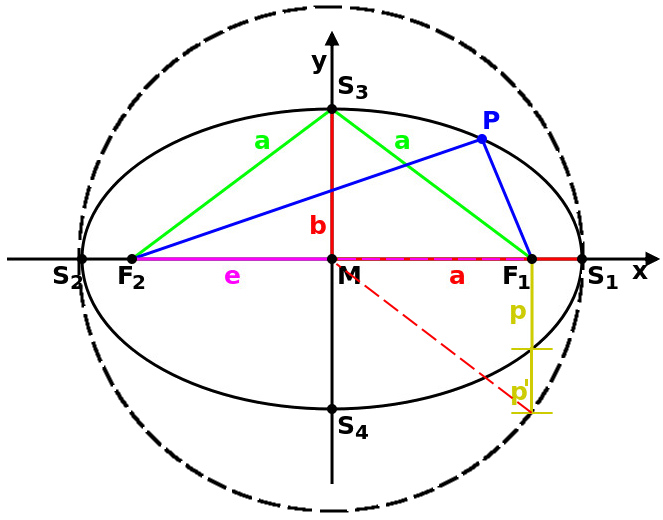
\includegraphics[width=0.6\textwidth]{./images/ellipse_new.jpg}                         %%
	\caption[Ellipse]{Ellipse, Quelle: Wikipedia zusätzlich eigener Überarbeitung}          %%
	\label{fig:ellipse}                                                                     %%
\end{figure}                                                                              	%%
%%%%%%%%%%%%%%%%%%%%%%%%%%%%%%%%%%%%%%%%%%%%%%%%%%%%%%%%%%%%%%%%%%%%%%%%%%%%%%%%%%%%%%%%%%%%%%      
Die Strecke \ensuremath{\overline{MS_{1}}} ist gleich der Strecke \ensuremath{\overline{MS_{2}}}. Man spricht bei der Länge dieser Strecke von der \textbf{großen Halbachse a}. Beide Strecken ergeben zusammen die Hauptachse \ensuremath{\overline{S_{1}S_{2}}}. Analog gibt es hierzu die Nebenachse, welche durch die Strecke \ensuremath{\overline{S_{3}S_{4}}} bestimmt wird. Die \textbf{kleinen Halbachsen} sind \ensuremath{\overline{MS_{3}}} und \ensuremath{\overline{MS_{4}}}. Diese haben die Längen \textbf{b}. Eine Ellipse kann auch als Stauchung eines Kreises mit dem Faktor \ensuremath{\frac{b}{a}} angesehen werden. 
\newpar
Die numerische Exzentrizität e' ist ein Maß für die Schlankheit der Ellipse. Sie ist definiert als
\begin{equation}
	e'=\frac{e}{a}
\end{equation}
Je größer die lineare Exzentrizität e im Verhältnis zu der großen Halbachse a wird, desto schlanker wird die Ellipse, da die Brennpunkte weiter vom Mittelpunkt entfernt sind. Das Wort numerisch gibt bei der Exzentrizität e' an, dass diese sich auf eine andere Größe (die große Halbachse) bezieht. Für eine Ellipse gilt \ensuremath{0 < e' < 1}. Für den Fall \ensuremath{e'=e=0} hat die Ellipse die selbe Erscheinung wie ein Kreis, da die Brennpunkte \ensuremath{F_1} und \ensuremath{F_2} im Mittelpunkt \ensuremath{M} liegen. Für \ensuremath{e'=1} entartet die Ellipse zu einer Geraden, da die kleine Halbachse b zu 0 wird. Um das zu zeigen wird die obige Gleichung noch mal herangezogen.
\begin{equation}
	e'^2=\frac{e^2}{a^2}=\frac{a^2-b^2}{a^2}=1-\left(\frac{b}{a}\right)^2 
	\label{equation_kepler_b}
\end{equation} 
\\Des Weiteren besitzt jede Ellipse einen Halbparameter \ensuremath{p}. Geht man davon aus, dass es einen Abstand \ensuremath{p'} gibt, welcher \ensuremath{p} bis zu einer die Ellipse umschließende Kreislinie verlängert, so gelten folgende Gleichungen
\begin{equation}
	\frac{p}{p'}=\frac{b}{a}
	\label{equation_kepler_p}
\end{equation}
Mit dem Satz eines alten Freudes folgt
\begin{equation}
p' = \sqrt{a^2-e^2}
\end{equation}
Jetzt ist klar, dass gilt
\begin{equation}
p=\frac{b}{a} \cdot p'= \frac{b}{a} \sqrt{a^2-e^2} = \frac{b^2}{a}
\label{equation_kepler_simple_p}
\end{equation}

Was nun noch fehlt ist „eine Gleichung, also eine analytische Beschreibung der Punkte einer Ellipse“ (siehe S.22 in \cite{Raumflugm}). Eine solche Gleichung ergibt sich mit dem Schnitt einer Ebene mit einem Kegel. 
%%%%%%%%%%%%%%%%%%%%%%%%%%%%%%%%%%%%%%%%%%%%%%%%%%%%%%%%%%%%%%%%%%%%%%%%%%%%%%%%%%%%%%%%%%%%%%
\begin{figure}[h]                                                                           %%
	\centering                                                                            	%%
	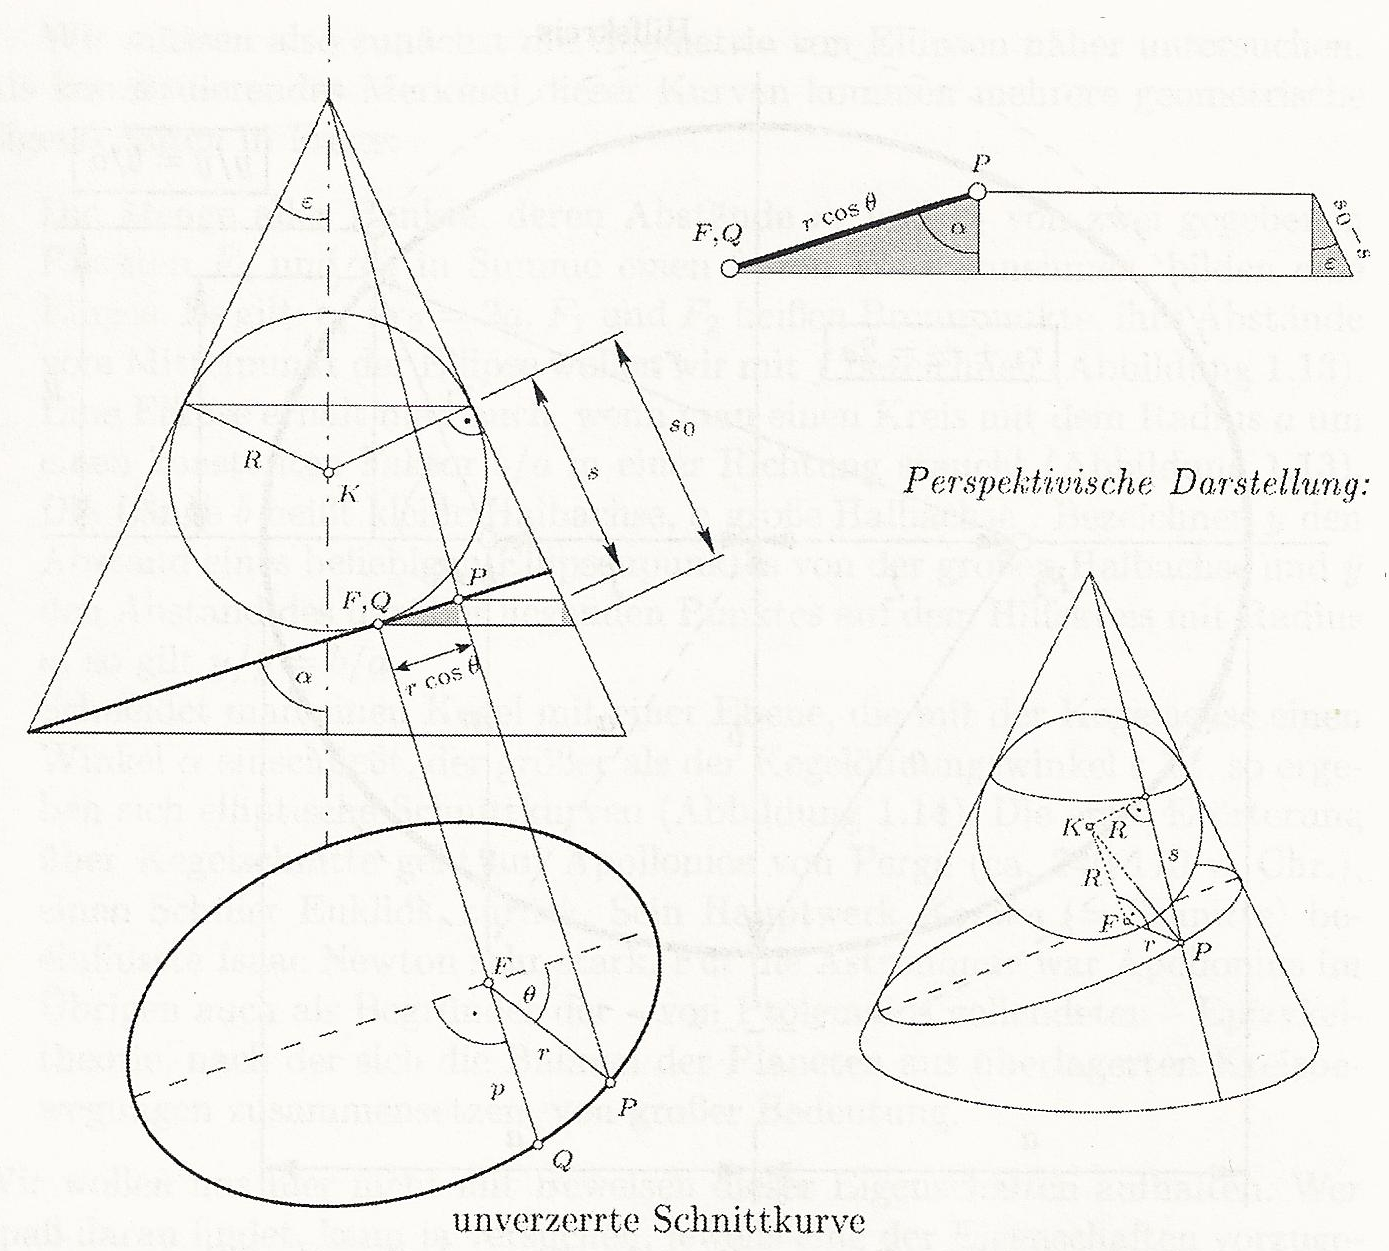
\includegraphics[width=0.8\textwidth]{./images/keplers_law1.jpg}                        %%
	\caption[Kegelschnitt]{Kegelschnitt, Quelle: S.24 in \cite{Raumflugm}}                  %%
	\label{fig:kegelsch_1}                                                                  %%
\end{figure}                                                                              	%%
%%%%%%%%%%%%%%%%%%%%%%%%%%%%%%%%%%%%%%%%%%%%%%%%%%%%%%%%%%%%%%%%%%%%%%%%%%%%%%%%%%%%%%%%%%%%%%      
Die Neigung der Schnittebene zur Kegelgrundfläche sei \ensuremath{\alpha}. Der Öffnungswinkel des Kegels sei \ensuremath{\epsilon}. Jetzt passiert etwas, dass das räumliche Denkvermögen herausfordert. In den Kegel wird eine (Dandelinsche) Kugel eingeschrieben. Diese Kugel berühre die Ebene im Punkt \ensuremath{F} und tangiere den Kegelmantel entlang eines Breitenkreises. Es ist einzusehen, dass der Punkt \ensuremath{F} auf der Hauptachse der Ellipse liegt. Der Schnittpunkt der entstehenden Ellipse und der Normale zur Hauptachse im Punkt \ensuremath{F} ist der Punkt \ensuremath{Q}. \ensuremath{P} stellt einen beliebigen Punkt auf der Ellipse dar. Die Verbindungslinie zwischen \ensuremath{F} und \ensuremath{P} hat zur Hauptachse die Neigung \ensuremath{\theta}. Der Abstand zwischen \ensuremath{F} und \ensuremath{P} ist \ensuremath{r}. \ensuremath{s} und \ensuremath{s_0} sind die Abstände der Punkte P und Q zum Berührkreis der Kugel gemessen entlang des Kegelmantels. 
\newpar
Man sieht nun, dass die Größen \ensuremath{r}, \ensuremath{s} und \ensuremath{\theta} von P abhängig sind. Es interessiere nun die mathematische Funktion \ensuremath{r(\theta)}, welche die Ellipsenbahn beschreibe (vgl. S.23 in \cite{Raumflugm}). Betrachtet wird nun zunächst die zweidimensionale Zeichnung rechts oben in Abb. \ref{fig:kegelsch}. Mit ein bisschen Nachdenken sieht man, dass
\begin{equation}
	(s_0-s) \cdot cos(\epsilon) = r \cdot cos (\theta) \cdot cos(\alpha)
	\label{equation1_kepler}
\end{equation} 
Doch woher kommt der Ausdruck \ensuremath{r \cdot cos(\theta)}? Hierzu werfe man einen Blick auf die zweidimensionale Abbildung der Schnittfläche/Ellipse links unten im Bild. Dieses Bild setze man nun in Relation zum Bild darüber. Der Abstand \ensuremath{r \cdot cos(\theta)} lässt sich nun auf die Hauptachse der Ellipse projizieren. \ensuremath{r}, die Projektionslinie für P die Hauptachse und F bilden nun eine rechtwinkliges Dreieck aus. Der Rest ist Trigonometrie. 
\newpar
In der Darstellung rechts unten in Abb. \ref{fig:kegelsch} ist folgende Beziehung auffindbar. 
\begin{equation}
 R^2 + s^2 = R^2 + r^2
\end{equation} 
Das bedeutet, dass \ensuremath{s} durch \ensuremath{r} in Gleichung \ref{equation1_kepler} ersetzt werden kann. 
\begin{equation}
	(s_0-r) \cdot cos(\epsilon) = r \cdot cos (\theta) \cdot cos(\alpha)
\end{equation}
Ausmultiplizieren ergibt
\begin{equation}
s_0 cos(\epsilon) - r cos(\epsilon) = r cos (\theta) cos(\alpha)
\end{equation}
Sortieren führt zu 
\begin{equation}
s_0 cos(\epsilon) = r cos (\theta) cos(\alpha) + r cos(\epsilon)
\end{equation}
Ausklammern und auflösen bringt
\begin{equation}
	r = \frac{s_0 cos(\epsilon) }{cos (\theta) cos(\alpha) + cos(\epsilon)}
		\label{equation2_kepler}
\end{equation}
Die entstandene Gleichung \ref{equation2_kepler} kann nun noch durch die Zusammenhänge \ensuremath{p=s_0} (Halbparameter) und \ensuremath{e'=\frac{cos(\alpha)}{cos(\epsilon)}} vereinfacht werden (vgl. S. 24 in \cite{Raumflugm}). Hierzu dividiert man Gleichung \ref{equation2_kepler} durch \ensuremath{cos(\epsilon)}. 
\begin{equation}
r = \frac{s_0}{1+\frac{cos(\alpha)}{cos(\epsilon)}cos (\theta)} = \frac{p}{1 + e' cos(\theta)} 
\label{equation3_kepler}
\end{equation}
Fertig ist die mathematische Version des ersten Keplerschen Gesetzes. 

\subsubsection{Das zweite Keplersche Gesetz}
%%%%%%%%%%%%%%%%%%%%%%%%%%%%%%%%%%%%%%%%%%%%%%%%%%%%%%%%%%%%%%%%%%%%%%%%%%%%%%%%%%%%%%%%%%%%%%
\begin{figure}[h]                                                                           %%
	\centering                                                                            	%%
	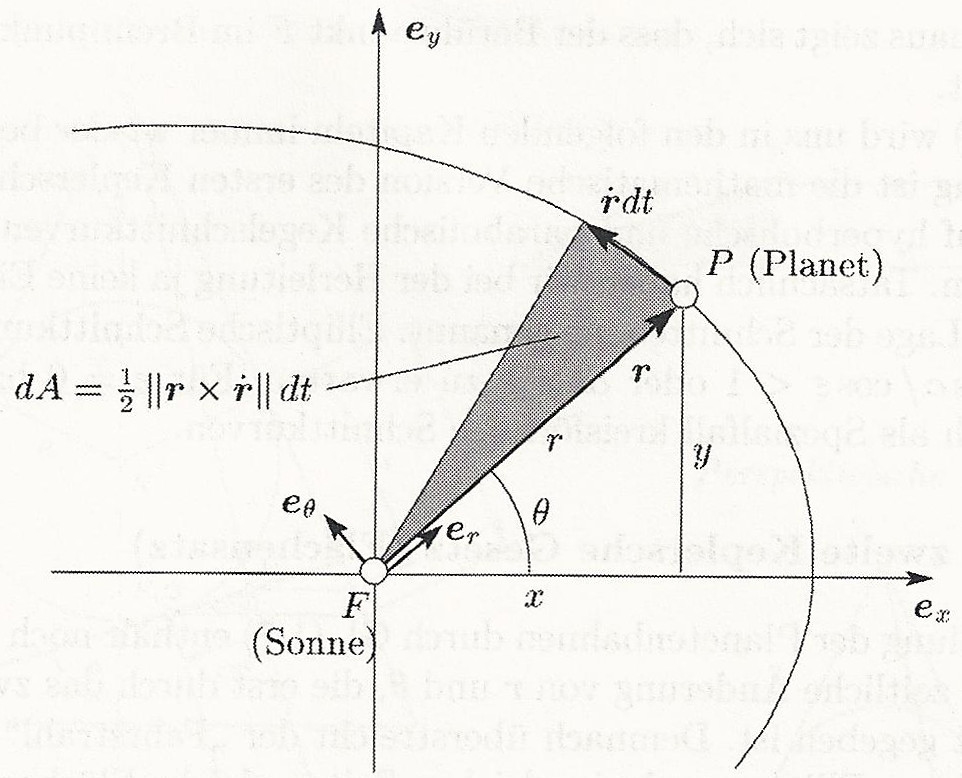
\includegraphics[width=0.6\textwidth]{./images/keplers_law2.jpg}                        %%
	\caption[Kegelschnitt]{Kegelschnitt, Quelle: S.26 in \cite{Raumflugm}}                  %%
	\label{fig:kegelsch_2}                                                                  %%
\end{figure}                                                                              	%%
%%%%%%%%%%%%%%%%%%%%%%%%%%%%%%%%%%%%%%%%%%%%%%%%%%%%%%%%%%%%%%%%%%%%%%%%%%%%%%%%%%%%%%%%%%%%%%      
Gleichung \ref{equation3_kepler} liefert noch keine Aussage über die zeitliche Änderung von \ensuremath{r} und \ensuremath{\theta}. Um eine Aussage über die zeitliche Änderung dieser Variablen treffen zu können, kann Keplers zweites Gesetz herangezogen werden: Die Fläche, welche die Verbindungslinie zwischen Sonne und einem Planet überstreicht ist zeitlich konstant. Die Fläche \ensuremath{\Delta A}, die in einem Zeitintervall \ensuremath{\Delta t} durch strichen wird ist genau
\begin{equation}
	\Delta A = \frac{1}{2}\left| \vec{r} \times \dot{\vec{r}} \right|\Delta t + F(\Delta t^2)
\end{equation}   
Die beiden Vektoren \ensuremath{r} und \ensuremath{\dot{r} \Delta t} spannen eine Fläche auf, welche ein Parallelogramm beschreibt. Das Kreuzprodukt ergibt einen Vektor dessen Länge dieser Fläche entspricht. Die Hälfte davon ist die Fläche des Dreiecks, die gesucht wird. Der Ausdruck \ensuremath{\dot{r} \Delta t} ist dabei sehr ungenau und beschreibt eigentlich nur die Änderung des Vektors \ensuremath{r}. Aus diesem Grund kommt noch der Fehlerterm \ensuremath{F} hinzu, der die Krümmung der Ellipse berücksichtigt. Bezieht man sich im nächsten Schritt auf infinitesimale Elemente, die wirklich gegen Null gehen, so erreicht man die gewünschte Genauigkeit. Der Fehlerterm wird überflüssig.  
\begin{equation}
dA = \frac{1}{2}\left| \vec{r} \times \dot{\vec{r}} \right|d t 
\label{equation_dA_kepler}
\end{equation}  
Man führt nun eine für jeden Planeten individuelle Konstante \ensuremath{h} ein, da sich das Verhältnis \ensuremath{\frac{dA}{dt}} nicht verändern darf. 
\begin{equation}
2 dA = h \cdot dt 
\end{equation}  
Um das mathematische Äquivalent zu dem sprachlich formulierten zweiten Gesetz zu erhalten, soll wie beim ersten Gesetz eine Abhängigkeit zu \ensuremath{r} und \ensuremath{\theta} hergestellt werden. Zu diesem Zweck wird die Gleichung einer Koordinatentransformation in Zylinderkoordinaten unterworfen (vgl. S. 25 f. in \cite{Raumflugm}). Es gilt also 
\begin{center}
	\ensuremath{x= r\, cos (\theta)}, \ensuremath{y=r\, sin (\theta)} und \ensuremath{z=z}. 
\end{center}
Gemäß der Definition von Zylinderkoordinaten darf man jetzt den Vektor \ensuremath{\vec{r}} auch anders schreiben:
\begin{equation}
	\vec{r} = r\,\vec{e_{r}} + z\,\vec{e_z}
\end{equation}
wobei folgendes generell über Zylinderkoordinatensysteme bekannt ist:
\begin{center}
	\ensuremath{\vec{e_{r}}=\left(\begin{array}{c}cos(\theta)\\ sin(\theta)\\0\end{array}\right)}, \ensuremath{\vec{e_{\theta}}=\left(\begin{array}{c}-sin(\theta)\\ cos(\theta)\\0\end{array}\right)}  und \ensuremath{\vec{e_z}=\left(\begin{array}{c}0\\0\\1\end{array}\right)}
\end{center}
Die Vektoren stehen allesamt senkrecht aufeinander, was man sieht, wenn man das Skalarprodukt bildet. Das liegt daran, dass das Skalarprodukt über die Summe der Längen der Vektoren multipliziert mit dem Kosinus des Winkels den sie einschließen definiert wird, welcher bei \ensuremath{\frac{\pi}{2}} bekanntlich Null ist.Da auch die Ableitung des Vektors \ensuremath{\vec{r}} (Geschwindigkeit) gesucht ist beginnt man zu differenzieren. Man wende hier zunächst die Summenregel, dann auf den ersten Ausdruck noch die Produkt- und die Kettenregel, da \ensuremath{\vec{e_{r}}} von \ensuremath{\theta} abhängt und diese wiederum von \ensuremath{t}. Es folgt
\begin{equation}
	\dot{\vec{r}} = \dot{r}\,\vec{e_r} + r\,\dot{\vec{e_r}} + \dot{z}\,\vec{e_z}
	\label{equation4_kepler}
\end{equation}
Setzt man nun   
\begin{center}	
	\ensuremath{\dot{\vec{e_{r}}}=\dot{\theta}\,\left(\begin{array}{c}-sin(\theta)\\ cos(\theta)\\0\end{array}\right)=\dot{\theta}\,\vec{e_{\theta}}}
\end{center}
in Gleichung \ref{equation4_kepler} ein, so ergibt sich  
\begin{equation}
\dot{\vec{r}} = \dot{r}\,\vec{e_r} + r\,\dot{\theta}\,\vec{e_{\theta}} + \dot{z}\,\vec{e_z}
\label{equation5_kepler}
\end{equation}
Man wählt nun die z-Achse geschickt, so dass diese senkrecht auf der Trägerebene der Ellipse steht (vgl. S.26 in \cite{Raumflugm}). Durch diesen Schachzug gilt für die zu betrachtenden Gleichungen \ensuremath{z=0}. Jetzt fällt Gleichung \ref{equation_dA_kepler} in sich zusammen
\begin{equation}
\frac{dA}{dt} = \frac{1}{2}\left| \vec{r} \times \dot{\vec{r}} \right| = \frac{1}{2}\left| r\,\vec{e_r} \times \left(\dot{r}\,\vec{e_r} + r\,\dot{\theta}\,\vec{e_{\theta}}\right) \right| 
\end{equation}  
Durch die Bilinearität des Kreuzprodukts folgt
\begin{equation}
\frac{dA}{dt} = \frac{1}{2}\left| \dot{r}\,r\,\left(\vec{e_r} \times \vec{e_r}\right) + r\,r\,\dot{\theta}\,\left(\vec{e_r} \times \vec{e_{\theta}}\right) \right| 
\end{equation}
Die Tatsache, dass das Kreuzprodukt eines Vektors mit sich selbst den Nullvektor ergibt und dem Umstand, dass \ensuremath{\vec{e_r}\perp\vec{e_\theta}\perp\vec{e_z}} ist, führt zu
\begin{equation}
\frac{dA}{dt} = \frac{1}{2}\left|r^2\,\dot{\theta}\,\vec{e_z} \right| =  \frac{1}{2}\,r^2\,\dot{\theta}=h=konstant
\label{equation6_kepler}
\end{equation}

\subsubsection{Das dritte Keplersche Gesetz}
Auf sein drittes Gesetz soll Kepler besonders stolz gewesen sein (vgl. S.27 in \cite{Raumflugm}). Nach seinem Gesetz stehen die Halbachsen \ensuremath{a_1} und \ensuremath{a_2} und die Umlaufzeiten \ensuremath{T_1} und \ensuremath{T_2} in dem Zusammenhang
\begin{equation}
	\frac{T_1^2}{T_2^2}=\frac{a_1^3}{a_2^3}
	\label{equation7_kepler}
\end{equation} 
Die Umlaufzeit lässt sich nun leicht mit der Konstanten \ensuremath{h}, welche für das zweite Keplersche Gesetz eingeführt wurde ausdrücken. Es wird hierfür die gesamte Ellipsenfläche (\ensuremath{A_{Ellipse}=ab\pi}) und konsequenterweise dann auch die gesamte Umlaufzeit \ensuremath{T} angenommen. Eingesetzt in Gleichung \ref{equation6_kepler} ergibt sich
\begin{equation}
	2ab\pi=hT.
\end{equation} 
Daraus folgt
\begin{equation}
	T=\frac{2ab\pi}{h}.
	\label{equation8_kepler}
\end{equation}
Eingesetzt in Gleichung \ref{equation7_kepler} ergibt sich 
\begin{equation}
		\frac{T_1^2}{T_2^2}=\frac{a_1^3}{a_2^3}=\frac{a_1^2b_1^2h_2^2}{a_2^2b_2^2h_1^2}.
\end{equation}
Bringt man nun \ensuremath{a_1^2b_1} und \ensuremath{a_2^2b_2^2} einmal durch Division und einmal durch Multiplikation eins weiter nach links, so kann man die Beziehung aus Gleichung \ref{equation_kepler_simple_p} ausnutzen und schreiben
\begin{equation}
\frac{a_1b_2^2}{a_2b_1^2}=\frac{h_2^2}{h_1^2}
\end{equation}
Oben und unten multipliziert man jetzt noch jeweils mit \ensuremath{1/a_1} und \ensuremath{1/a_2}.
\begin{equation}
\frac{b_2^2/a_2}{b_1^2/a_1}=\frac{h_2^2}{h_1^2}=\frac{p_2}{p_1}
\end{equation}
Das Resultat ist ein „Zusammenhang zwischen den Halbparametern \ensuremath{p_1}, \ensuremath{p_2} und den Bewegungskonstatnten \ensuremath{h_1}, \ensuremath{h_2}“ (siehe S.27 in \cite{Raumflugm}). Diese Größen sind aus dem zweiten Keplerschen Gesetz bekannt. 
\newpar
Die Bewegungskonstante \ensuremath{h} ist eine wichtige Größe, um die Umlaufzeit \ensuremath{T} und auch um die Mittlere Anomalie \ensuremath{M(t)} bzw. die Kreisfrequenz \ensuremath{n} dieser zu bestimmen. Um an diese Größe zu gelangen leitet man nach S.87 in \cite{HandRaum} aus der Zentrifugalkraft und der Gravitationskraft für einen Sonderfall das dritte Keplersche Gesetz her. Man tut so als bewege sich ein Körper mit der Masse \ensuremath{m_{Sat}} auf einer Kreisbahn mit dem Radius \ensuremath{a}, was für eine (numerische und lineare) Exzentrizität von 0 zutrifft. Da der Körper nicht ins Schwerezentrum im Mittelpunkt der Bahn abstürzt, muss die Gravitationskraft gleich der Zentrifugalkraft sein. Es folgt
\begin{equation}
	F_{Z}=F_{G}
\end{equation}     
\begin{equation}
	m_{Sat}\cdot n^2 \cdot a= G \cdot \frac{m_{Sat}\,M_{Erde}}{a^2}
\end{equation} 
\begin{equation}
	 a^3\,\left(\frac{2\pi}{T}\right)^2= G\,M_{Erde}
\end{equation}     
Aus dieser Gleichung folgt durch ein paar geschickte Umformungen, die aus Platzgründen an dieser Stelle nicht niedergeschrieben wurden, und Umstellen nach \ensuremath{T}
\begin{equation}
	T=\frac{2\,a^2\,\pi}{\sqrt{G\,M_{Erde}\,a}}
\end{equation}
Im Zähler steht die doppelte von der Verbindungslinie zwischen Schwerezentrum und Satellit in einer Umlaufperiode \ensuremath{T} überschrittenen Fläche. Durch die Verwandschaft der obigen Gleichung mit Gleichung \ref{equation8_kepler}, kann man schlussfolgern, dass die Bewegungskonstante in diesem Fall sich zu 
\begin{equation}
	h=\sqrt{G\,M_{Erde}\,a}
\end{equation}   
ergibt. Die Berechnung der mittleren Anomalie \ensuremath{M(t)} stellt nun kein Problem mehr da.
\subsection{Die Bahnelemente}
%%%%%%%%%%%%%%%%%%%%%%%%%%%%%%%%%%%%%%%%%%%%%%%%%%%%%%%%%%%%%%%%%%%%%%%%%%%%%%%%%%%%%%%%%%%%%%
\begin{figure}[h]                                                                           %%
	\centering                                                                            	%%
	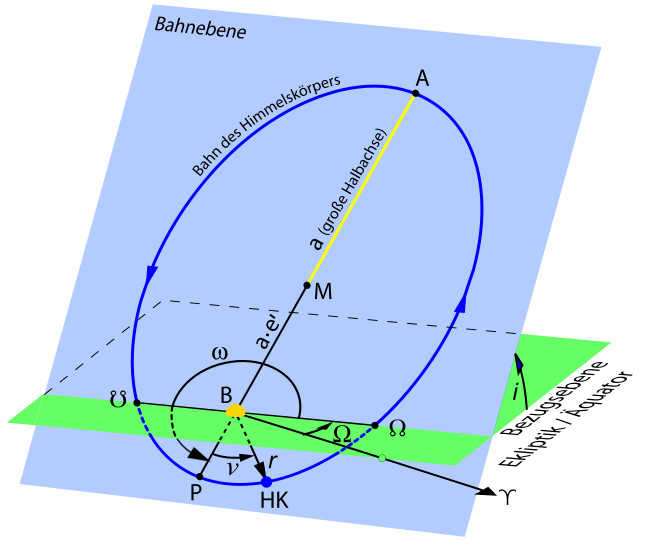
\includegraphics[width=0.8\textwidth]{./images/bahnelemente.jpg}                        %%
	\caption[Bahnelemente]{Bahnelemente, Quelle: \cite{Wiki:Bahnel}, 
		Grafik ist eigens modifiziert}              
	\label{fig:bahnelemente}                                                                %%
\end{figure}                                                                              	%%
%%%%%%%%%%%%%%%%%%%%%%%%%%%%%%%%%%%%%%%%%%%%%%%%%%%%%%%%%%%%%%%%%%%%%%%%%%%%%%%%%%%%%%%%%%%%%%   
Die Bahnelemente dienen der Beschreibung einer Bewegung eines Himmelskörpers auf einer Umlaufbahn (meist einer Ellipse). Dieser Körper unterliegt den Keplerschen Gesetzen. Wird die Bewegung eines Himmelskörpers durch äußere Einflüsse (z.B. Gravitationskraft der Sonne) nicht gestört, so kann sie durch sechs Größen beschrieben werden. Diese Größen sind die Bahnelemente. Zwei Bahnelemente beschreiben die \textbf{Form der Bahn}, drei legen die \textbf{Lage der Bahn} im dreidimensionalen Raum fest und ein Bahnelement gibt an zu welcher \textbf{Zeit} sich der Himmelskörper wo auf der Bahn befunden hat. 
\newpar
Diese Bahnelemente reichen in der Praxis nicht aus, um die Position eines Himmelskörpers z.B. eines Satelliten mit einem Vorhersagemodell berechnen zu können. Aus diesem Grund werden die Bahnelemente meist um von Vorhersagemodellen benötigten Informationen ergänzt.       
Im Folgenden werden die Bahnelemente in Ihrer Bedeutung anhand der Abbildung \ref{fig:bahnelemente} erläutert. 

\subsubsection{Gestalt der Bahn}
Um die Gestalt der Bahn zu beschreiben wird die \textbf{numerische Exzentrizität (1) \ensuremath{e'}} und die Angabe der Länge der \textbf{großen Halbachse (2) \ensuremath{a}} benötigt. Diese beiden Größen werden ausführlich im Absatz \ref{subsec:kepler} beschrieben. Es braucht nicht mehr, um eine elliptische Bahn zu definieren. Zur Erinnerung: Die große Halbachse \ensuremath{a} ist die Länge der Strecke vom Mittelpunkt zu den Hauptscheiteln. Die (lineare) Exzentrizität \ensuremath{e} gibt die Schlankeit der Ellipse an. Wobei die numerische Exzentrizität \ensuremath{e'} auf die große Halbachse normiert ist.  
\newpar
Die Abhängigkeit der Umlaufzeit eines Satelliten von den Bahndimensionen (v.a. Länge der großen Halbachse ) und die elliptische Bahnform sind der „quadratischen Abnahme der Gravitationsbeschleunigung [geschuldet]“ (siehe S. 87 in \cite{HandRaum}). 
\begin{equation}
\ddot{\vec{r}}=-\frac{GM_{Erde}}{r^2}\cdot\frac{\vec{r}}{r}
\end{equation}    
\ensuremath{GM_{Erde} \approx 398600,4\,\frac{km^3}{s^2}} ist dabei das konstante Produkt aus Gravitationskonstante und Masse der Erde. Das Stichwort lautet hier Impulserhaltungssatz. In einem geschlossenen System kann Impuls weder vernichtet noch erschaffen werden. Bis zum Perigäumsdurchgang nimmt ein Satellit Impuls von der Erde über die Kraft, die zum Erdmittelpunkt hin wirkt auf. Danach wird Impuls an dier Erde abgegeben \ensuremath{\rightarrow} der Satellit verlangsamt sich. Nach dem Apogäumsdurchgang fängt der Satellit wieder an schneller zu werden. Er nimmt wieder Impuls auf.  
  
\subsubsection{Lage der Bahn}
Es erscheint sinnvoll, dass die Lage im Raum als nächstes festgelegt wird. Auch scheint es sinnig, dass man drei Bahnellemente benötigt, um die Lage der Bahn im dreidimensionalen Raum festzulegen. 
\newpar
Man stelle sich nun vor, dass die Ellipse, auf welcher der Satellit sich bewegt, in einer Ebene liege.  Diese Ebene schneide man mit einer Referenzebene (z.B. Schnittebene durch den Erdäquator). Die \textbf{Inklination (3) \ensuremath{i}} ist nun ein Winkel, „um den die Bahnebene gegenüber der [Referenzebene] geneigt ist“ (siehe S.88 in \cite{HandRaum}). Um die Nebenachse der Ellipse herum kann durch diese Festlegung keine Rotation mehr stattfinden. Die Ellipse, die ja in der Ebene liegt, kann sich jetzt noch in dieser Ebene um eine zur Ebene orthogonalen Achse drehen. Um das zu unterbinden wird ein weiterer Winkel, das \textbf{Argument des Perigäums (4) \ensuremath{\omega}}, eingeführt. Das Argument des Perigäums ist der Winkel, den die Knotenlinie und die Perigäumsrichtung (Hauptachse) einschließen. Das Perigäum liegt am Ende der Hauptachse, auf welches sich der Satellit zu bewegt, nachdem er den aufsteigenden Knoten passiert hat. Der aufsteigende Knoten ist der Punkt in dem der Satellit die Referenzebene auf seiner elliptischen Umlaufbahn (von Süd nach Nord) durchstößt. Die Knotenlinie ist die Schnittgerade der Ellipse mit der Referenzebene. Darüber hinaus gibt es das Apogäum, welches nach dem absteigenden Knoten durchlaufen wird, der am anderen Ende der Nebenachse beheimatet ist. Eine andere Definition für das Perigäum ist der Punkt des geringsten Abstands des Satelliten zur Erde. Analog lässt sich das Apogäum als Punkt des größten Abstands des Satelliten zur Erde festlegen. Die Ellipse dreht sich nun nicht mehr in der Ebene. Eine Sache wurde jetzt noch nicht betrachtet. Die Ebene kann sich immer noch entlang Ihrer Hauptachse drehen. Die \textbf{Rektaszension des aufsteigenden Knotens (5) \ensuremath{\Omega}} gibt nun den Winkel an, den die Knotenlinie und der Vektor vom Ellipsenmittelpunkt zum Frühlingspunkt \ensuremath{\gamma} einschließen. Doch was ist der Frühlingspunkt? „Als Frühlingspunkt (auch Widderpunkt) wird in der Astronomie der Schnittpunkt des Himmelsäquators mit der Ekliptik bezeichnet, an dem die Sonne zum Frühlingsanfang der Nordhalbkugel (= Herbstanfang der Südhalbkugel) steht“ (siehe \cite{Wiki:Frue}). Die Derehung um die Hauptachse ist jetzt also auch nicht mehr möglich. Der Bahnlage wurden somit alle drei Freiheitsgrade genommen.     
\newpar
Die Bewegung eines Satelliten erfolgt in einer nicht veränderbaren Bahnebene mit dem Bahnmittelpunkt gleich dem Erdmittelpunkt. Dies impilziert das erste Keplersche Gesetz. Der Grund hierfür ist „dass die Anziehung der Erde (in erster Näherung) immer zum Erdmittelpunkt gerichtet ist“ (siehe S. 87 in \cite{HandRaum}). Zu keinem Zeitpunkt gibt es somit einen Kraftvektor, der Senkrecht zum Ortsvektor \ensuremath{\vec{r}} wirkt und somit die Bahnebene verschieben könnte (Annahme: Mittelpunkt des Koordinatensystems ist der Erdmittelpunkt). Daraus resultiert wiederum, dass eine einmal eingeschlagene Bahnebene ohne eine äußere Kraft nicht wieder verlassen werden kann.
 
\subsubsection{Zeitlicher Bezug und Kepler-Gleichung}
Bis jetzt ist alles recht schön und anschaulich. Es ist klar wo die Bahnebene im Raum ist und wie diese aussieht. Wir haben durch das zweite Keplersche Gesetz eine Gleichung, die uns die Position des Satelliten in Abhängigkeit des Winkels \ensuremath{\theta} verrät. Diese ist 
\begin{equation}
	r = \frac{p}{1 + e' cos(\theta)} 
\end{equation}
\ensuremath{\theta} ist der Winkel, den die Verbindungslinie zwischen einem Brennpunkt und dem Satellit mit der Hauptachse einschließt. Es gibt allerdings noch ein Haar in der Suppe. Aufgrund des Flächensatzes ist die Winkelgeschwindigkeit des Satelliten nicht konstant (bzw. nur für eine in der Natur nicht vorkommende Kreisbahn konstant). \ensuremath{\theta} ist eine Funktion von \ensuremath{t}. Die sog. wahre Anomalie \ensuremath{\theta(t)} schwankt um die mittlere Anomalie \ensuremath{M} (nicht zu verwechseln mit der Erdmasse). Man stößt nun auf das Zweikörperproblem (Keplerproblem). Dies ist die Angabe der wahren Anomalie \ensuremath{\theta(t=t_x)} zu einem vorgegebenen Zeitpunkt \ensuremath{t_x}.  Wie kommt die mittlere Anomalie nun zustande? Zunächst sollte ein genauer Blick auf Abbildung \ref{fig:kepler_gl} geworfen werden. Die Abbildung stellt eine Momentaufnahme einer Situation dar.     
%%%%%%%%%%%%%%%%%%%%%%%%%%%%%%%%%%%%%%%%%%%%%%%%%%%%%%%%%%%%%%%%%%%%%%%%%%%%%%%%%%%%%%%%%%%%%%
\begin{figure}[h]                                                                           %%
	\centering                                                                            	%%
	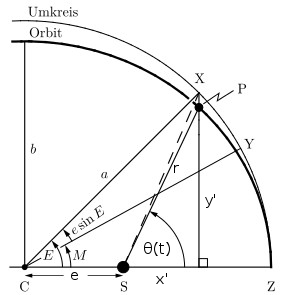
\includegraphics[width=0.4\textwidth]{./images/keplers_equation.jpg}                    %%
	\caption[Kepler-Gleichung]{Kepler-Gleichung, Quelle: \cite{Wiki:KeplerGl}, 
								Grafik ist eigens modifiziert}              				%%
	\label{fig:kepler_gl}                                                                	%%
\end{figure}                                                                              	%%
%%%%%%%%%%%%%%%%%%%%%%%%%%%%%%%%%%%%%%%%%%%%%%%%%%%%%%%%%%%%%%%%%%%%%%%%%%%%%%%%%%%%%%%%%%%%%%   
Wie schon bei früheren Betrachtungen wird die Ellipse (Orbit) in einen Umkreis eingeschrieben. Ein fiktiver (mittlerer) Satellit \ensuremath{Y} laufe entlang des Umkreises um den Punkt \ensuremath{C} (Mittelpunkt der Ellipse und des Kreises, kein Ellipsenbrennpunkt). Der wahre Satellit \ensuremath{P} bewege sich entlang der Ellipse. Die Lage des fiktiven Satelliten \ensuremath{Y} wird zum Zeitpunkt \ensuremath{t} mittels des Winkels \ensuremath{M} dargestellt. Hierbei wird unterstellt, dass der Satellit zum Zeitpunkt \ensuremath{t_P} im Perigäum (oft auch Periapsis genannt) \ensuremath{M=0} war. Es gilt nun
\begin{equation}
	M=2\pi\,\frac{t-t_P}{T}=n\,(t-t_P)
\end{equation}   
Hierbei ist \ensuremath{n} die Winkelgeschwindigkeit und \ensuremath{T} die Umlaufzeit des Satelliten um das Schwerezentrum. \ensuremath{S} ist der Erdmittelpunkt (Schwerezentrum). 
Um nun die Kurve zu der Ellipse und dem tatsächlichen Satellit zu erhalten wird das zweite Keplersche Gesetz für diesen konkreten Fall herangezogen. In gleichen Zeiträumen werden gleiche Flächen von den Fahrstrählen der Satelliten unabhängig von der Bahnform (egal ob elliptisch oder kreisförmig mit \ensuremath{e'=e=0}) überstrichen. Hier spricht man von einer bijektiven Abbildung der Ellipsen- und Kreisflächensegmente. Letztere sind leicht zu berechnen. Es wird also praktisch ein Umweg über den Umkreis gegangen. Das zweite Keplersche Gesetz angewandt auf den vorliegenden Fall, führt bezüglich der Zeitspanne einer Überstreichung der gesamten Fläche zu
\begin{equation}
	\frac{A_{Kreis}}{A_{Ellipse}}=\frac{\pi\,a^2}{\pi\,a\,b}
\end{equation}
Nach dem zweiten Keplerschen Gesetz ist dieses Vehätlnis dasselbe für eine infinitesimale Fläche. So gilt
\begin{equation}
	\frac{A_{CYZ}}{A_{SPZ}}=\frac{A_{Kreis}}{A_{Ellipse}}=\frac{a}{b}
	\label{equation1_kepler_equ}
\end{equation}
\newpar
Kepler führte als eine Hilfsgröße die exzentrische Anomalie \ensuremath{E} ein. Hierzu wird \ensuremath{P} auf den Hilfskreis projeziert. Es entsteht der Punkt \ensuremath{X}. Der Winkel zwischen Hauptachse und \ensuremath{X} ist die exzentrische Anomalie. Durch den in Gleichung \ref{equation1_kepler_equ} hergeleiteten Zusammenhang kann folgende Aussage getroffen werden. 
\begin{equation}
	A_{SXZ}=\frac{a}{b}A_{SPZ}	
	\label{equation2_kepler_equ}
\end{equation}  
Setzt man Gleichung \ref{equation1_kepler_equ} in Gleichung \ref{equation2_kepler_equ} ein, so ergibt sich
\begin{equation}
	A_{SXZ}=A_{CYZ}	
	\label{equation3_kepler_equ}
\end{equation}
Mit der Gleichung \ref{equation3_kepler_equ} ist ein indirekter Zusammenhang zwischen der mittleren Anomalie (Punkt \ensuremath{Y}) und der exzentrischen Anomalie (Punkt \ensuremath{X}) gefunden. Der Fahrstrahl \ensuremath{\overline{CY}} in der Zeit einer Periode \ensuremath{U} eine Fläche von \ensuremath{\pi\,a^2} überstreicht, so überstreicht er in einer Zeit \ensuremath{t} eine Fläche, die um den Faktor \ensuremath{\frac{M}{2\,\pi}} kleiner ist. Es folgt 
\begin{equation}
	A_{CYZ}=\frac{M}{2\,\pi}\,\pi\,a^2=\frac{a^2}{2}M	
	\label{equation4_kepler_equ}
\end{equation}  
Analog gilt dies für den Fahrstrahl \ensuremath{\overline{CX}}.
\begin{equation}
	A_{CXZ}=\frac{a^2}{2}E	
	\label{equation5_kepler_equ}
\end{equation}
Weiter geht's mit noch mehr Geometrie. Die Fläche \ensuremath{A_{CXZ}} kann in zwei Teilflächen zerlegt werden.
\begin{equation}
	A_{CXZ}=A_{CSX}+A_{SXZ}
	\label{equation6_kepler_equ}
\end{equation}
Die Fläche \ensuremath{A_{CSX}} kann als die Fläche eines Dreiecks aufgefasst werden. Dabei ist \ensuremath{a\cdot e'} die Basis und \ensuremath{a\,sin(E)} die Höhe des Dreiecks. 
\begin{equation}
	A_{CSX}=\frac{1}{2}\cdot a\cdot e' \cdot a\,sin(E)=\frac{a^2}{2}\,e'\,sin(E)
	\label{equation7_kepler_equ}
\end{equation}
Als letzten Schritt setze man nun noch Gleichung \ref{equation3_kepler_equ} (unter Beachtung von Gleichung \ref{equation4_kepler_equ}), Gleichung \ref{equation5_kepler_equ} und Gleichung \ref{equation7_kepler_equ} in Gleichung \ref{equation6_kepler_equ} ein.
\begin{equation}
	\frac{a^2}{2}E=\frac{a^2}{2}\,e'\,sin(E)+\frac{a^2}{2}M
	\label{equation8_kepler_equ}
\end{equation}
Mit ein paar Tricks aus der Grundschule entsteht die \textbf{Kepler-Gleichung} wie sie im Buche steht.
\begin{equation}
	E-e'\,sin(E)=M=n\cdot (t-t_P)
	\label{equation_kepler_equ_final}
\end{equation}
Diese Gleichung kann nicht nach \ensuremath{E} aufgelöst werden und so keine schöne Funktion \ensuremath{E(t)} gewonnen werden. Doch Gott sei dank, schenke er Newton die Eingebung des Newton-Verfahrens zur Nullstellensuche. Das Newton-Verfahren ist im Grunde eine rekursive Folge, wobei jedes Folgeglied allgemein mit
\begin{equation}
	x_{n+1}=x_n-\frac{f(x_n)}{f'^{x}(x_n)}
	\label{equation9_kepler_equ}
\end{equation}
zu bestimmen ist. Man stellt also Gleichung \ref{equation_kepler_equ_final} entsprechend um und leite ab.
\begin{equation}
	f(E)=E-e'\,sin(E)-M \stackrel{!}{=} 0
	\label{equation10_kepler_equ}
\end{equation}
\begin{equation}
	f'^{E}(E)=1-e'\,cos(E) 
	\label{equation11_kepler_equ}
\end{equation}
Es folgt die rekursive Folge für die Kepler-Gleichung. 
\begin{equation}
	E_{n+1}=E_n-\frac{E-e'\,sin(E)-M}{1-e'\,cos(E) }
	\label{equation12_kepler_equ}
\end{equation}
Als Startwert wird in \cite{HandRaum} \ensuremath{E_0=M} empfohlen. Die rekursive Folge Verhält sich dabei so, dass sie gegen einen entsprechenden Wert für die exzentrische Anomalie \ensuremath{E} konvergiert. Wenn sich entsprechende Nachkommastellen nach gewisser Genauigkeit nicht mehr ändern, so hat man die Nullstelle gefunden. Mit diesem Wert für \ensuremath{E(t=t_x)} kann die wahre Anomalie \ensuremath{\theta(t=t_x)} bestimmt werden. Zu beachten ist, dass in die Kepler-Gleichung natürlich vor der Anwendung des Newton-Verfahrens auch der gewünschte Zeitpunkt \ensuremath{t_p} eingesetzt wird.     
\newpar
Wie bestimmt man nun die wahre Anomalie, also den Winkel, der zu dem Zeitpunkt gehört aus welchem wir dann wiederum einen Vektor \ensuremath{r} gewinnen können? Hierzu werden die Größen \ensuremath{x'} und \ensuremath{y'} in Abbildung \ref{fig:kepler_gl} herangezogen. Man sucht nun nach einer Beziehung zwischen diesen Größen und bekannten Größen aus dem Fundus der Bahnelemente die Form der Bahn betreffend (dazu gehören natürlich auch abgeleitete Größen). 
Es ist nachvollziehbar, dass 
\begin{equation}
	x'=r\,cos(\theta)=cos(E)\,a-e=a\left(cos(E)-e'\right)
\end{equation}
ist. Für \ensuremath{y'} muss man etwas tiefer in die Trickkiste greifen. Man geht aus von Gleichung \ref{equation_kepler_p}. Diese stelle man nach \ensuremath{p} um.
\begin{equation}
	p=p'\,\frac{b}{a}
\end{equation} 
Für \ensuremath{p'} kann der Term \ensuremath{sin(E)\,a} eingesetzt werden. Mit dem Satz des Pythagoras kann \ensuremath{b} auch mit den größen \ensuremath{a} und \ensuremath{e} ausgedrückt werden. Es folgt  
\begin{equation}
	p=y'=sin(E)\,a\,\frac{\sqrt{a^2-e^2}}{a}=sin(E)\,a\,\sqrt{1-e'^2}
\end{equation} 
Aus diesen beiden Größen kann unmittelbar die wahre Anomalie \ensuremath{\theta} zu einem gegebenen Zeitpunkt bestimmt werden.
\begin{equation}
	\theta=arctan\left(\frac{y'}{x'}\right)=arctan\left(\frac{sin(E)\,a\,\sqrt{1-e'^2}}{a\left(cos(E)-e'\right)}\right)=arctan\left(\frac{sin(E)\,\sqrt{1-e'^2}}{cos(E)-e'}\right)
\end{equation}
\newpar
Nun ist also der zeitliche Bezug bekannt. Hier nochmal eine kleine Darstellung wie vorzugehen ist.
\begin{center}
	\smartdiagram[circular diagram:clockwise]{\ensuremath{t} gegeben, \ensuremath{M=n\cdot (t-t_P)} bestimmen, \ensuremath{E} bestimmen, \ensuremath{x'} und \ensuremath{y'} bestimmen, \ensuremath{\theta} und \ensuremath{r} bestimmen} 
\end{center}
Führt man den Vorgang wie oben gezeigt iterativ aus, so erhält man einen zweidimensionalen Vektor \ensuremath{\vec{r}}. Wenn man nun scharf nachdenkt, so fällt einem auf, dass man nochmal eine Information benötigt. Es braucht einen Zeitpunkt \ensuremath{t_P}. Dies muss ein Zeitpunkt sein, bei welchem der Satelliten im Perigäum stand. Als Analogie könnte man die Phase eines Signals in der Elektrotechnik angeben. Genau diesen Zeitpunkt liefern die Bahnelemente als zeitlichen Bezug.
\newpar
Als Zusammenfassung hier nochmal eine Übersicht aller Bahnelemente. 
\begin{itemize}
	\item Gestalt der Bahn
	\begin{itemize}
		\item die große Halbachse \ensuremath{a}
		\item die numerische Exzentrizität \ensuremath{e'}
	\end{itemize}
	\item Lage der Bahn
	\begin{itemize}
		\item die Inklination \ensuremath{i}
		\item die Rektaszension des aufsteigenden Knotens \ensuremath{\Omega}
		\item das Argument des Perigäums \ensuremath{\omega}
	\end{itemize}
	\item Zeitlicher Bezug
	\begin{itemize}
		\item die Epoche (wann ist der Sattelit im Perigäum gewesen) \ensuremath{t_P}
	\end{itemize}
\end{itemize} 

\subsection{Von den Bahnelementen zum Vektor}
Im nächsten Schritt trägt man alle Informationen aus den Bahnelementen zusammen, um einen Vektor \ensuremath{\vec{r}} im dreidimensionalen kartesischen Koordinatensystem zu erhalten. Der Ursprung des Koordinatensystems soll im Erdzentrum liegen und der Vektor \ensuremath{\vec{r}} soll ein Ortsvektor des Satelliten sein. Die x-y-Ebene dieses Koordinatensystems ist der Äquator. Das Ergebnis der bisherigen Berechnungen ist der Vektor
\begin{equation}
	\vec{r'}=a\cdot\left(\begin{array}{c}cos(E)-e'\\ sin(E)\,\sqrt{1-e'^2} \\0\end{array}\right)
\end{equation}
Die Satellitenbahn liegt nach der obigen Gleichung in der äquatorialen Ebene. Der Erdmittelpunkt liegt im Brennpunkt der Ellipse. Anstatt die Bahnebene zu drehen. Dreht man nun das Koordinatensystem. Allerdings in die mathematisch entgegengesetzte Richtung. Hierfür können natürlich nur die Winkel verwendet werden, welche in den Bahnelementen für die Lage der Bahn mitgeliefert werden. Bei der Drehung wird auf Drehmatrizen zurückgegriffen. Eine gute Veranschaulichung dieser Drehungen findet man \href{https://www.youtube.com/watch?v=QZrYaKwZwhI}{\textit{in dieser Animation}}. Der gesuchte Vektor ergibt sich nun zu
\begin{equation}
	\vec{r}=\mathbf{R_Z}(-\Omega)\,\mathbf{R_X}(-i)\,\mathbf{R_Z}(-\omega)\cdot a\cdot\left(\begin{array}{c}cos(E)-e'\\ sin(E)\,\sqrt{1-e'^2} \\0\end{array}\right) 
\end{equation}  
Hierbei stellen \ensuremath{\mathbf{R_X}} und \ensuremath{\mathbf{R_Z}} folgende Drehmatrizen dar (nachzuschlagen auf S.89 in \cite{HandRaum}). 
\begin{equation}
\mathbf{R_X}(\alpha) = 
	\left(
		\begin{array}{ccc}
			1 & 0 & 0 \\
			0 & +cos\,\alpha & +sin\,\alpha\\
			0 & -sin\,\alpha & +cos\,\alpha
		\end{array}
	\right)
\end{equation}
\begin{equation}
\mathbf{R_Z}(\alpha) = 
	\left(
		\begin{array}{ccc}
			+cos\,\alpha & +sin\,\alpha & 0\\
			-sin\,\alpha & +cos\,\alpha & 0\\
			0 & 0 & 1 \\
		\end{array}
	\right)
\end{equation}
Eine Frage, die sich aufdrängen mag ist: Warum kann die Drehung der Ellipse in der Bahnebene (Argument des Perigäums \ensuremath{\omega}) einfach auf eine Drehung der z-Achse zurüclgeführt werden? Man kann es sich auch so vorstellen, dass zunächst die Ellipse noch in der äquatorialen Ebene liegt, die z-Achse dann um \ensuremath{-\omega} gedreht wird, dann die x-Achse um \ensuremath{-i} und letztendlich die z-Achse nochmal um \ensuremath{-\Omega} gedreht wird.
\newpar
Nach \cite{HandRaum} ergibt sich nach der Ausführung der Drehungen der Vektor
\begin{equation}
\vec{r} = r\cdot  
	\left(
		\begin{array}{c}
				cos(\omega+\theta)\,cos(\Omega)-sin(\omega+\theta)\,cos(i)\,sin(\Omega)\\
				cos(\omega+\theta)\,sin(\Omega)+sin(\omega+\theta)\,cos(i)\,cos(\Omega)\\
				sin(\omega+\theta)\,sin(i)				
		\end{array}
	\right)
	\label{equation1_kep_elements}
\end{equation}
Durch Ableitung nach der Zeit kommt man wie in \cite{HandRaum} angegeben auf
\begin{equation}
	\vec{v}=\mathbf{R_Z}(-\Omega)\,\mathbf{R_X}(-i)\,\mathbf{R_Z}(-\omega)\cdot\frac{\sqrt{GM_{Erde}\,a}}{r}\cdot\left(\begin{array}{c}-sin(E)\\ cos(E)\,\sqrt{1-e'^2} \\0\end{array}\right) 
	\label{equation2_kep_elements}
\end{equation} 
Gleichung \ref{equation1_kep_elements} lässt sich so interpretieren, dass der Term \ensuremath{\sqrt{\frac{GM_{Erde}}{r^2\,a}}} die zeitliche Ableitung der exzentrischen Anomalie \ensuremath{E} sein muss, da die Kettenregel der Differentialrechnung greift und die Rotationsmatrizen keine zetilichen Abhängigkeiten aufweisen.
\newpar
Mit den Gleichungen \ref{equation1_kep_elements} und \ref{equation2_kep_elements} lässt sich nun die Antenne fast ausrichten und nachführen. Der nächste Schritt ist die Berücksichtigung der Position der Bodenstation auf der Erde. Um sich das Leben nicht unnötig schwer zu machen, verwendet geografische Koordinaten und gewinnt daraus einen Ortsvektor für das kartesische Koordinatensystem im Erdmittelpunkt. Es wird hierbei vernachlässigt, dass die Erde keine Kugel sondern annähernd ein Ellipsoid ist. Ganz korrekt würde man es machen, wenn man sich des World Geodetic System 1984 (WGS84) bedient. Laut \cite{Wiki:Geo} können durch diese Vernachlässigung Orstverschiebungen (der Bodenstation) von bis zu 20km auftreten. Es soll jedoch zunächst möglichst einfach verstanden werden, wie ein Programm wie GPredict vorgeht und auch zur Überprüfung der Daten, die GPredict liefert reicht die Genauigkeit aus, die mit dieser Vernachlässigung erreicht wird .
\newpar  
Im ersten Schritt zur  \textbf{Beschreibung der Bahn im erdfesten System} muss das Koordinatensystem nochmal an der z-Achse gedreht werden. Das liegt daran, dass die x-y-Ebene zwar im Äquator liegt, die x-Achse jedoch nicht auf den nullten Längengrad, sondern auf den Frühlingspunkt zeigt. Bei dieser Achsentransformation wird auch die Rotation der Erde mit berücksichtigt. Die x-Achse wird in den sog. Meridian von Greenwich gezogen. Die Drehung der z-Achse wird mit dem Winkel \ensuremath{\Theta} vollzogen. Dieser Winkel wird dabei als „Sternenzeit bezeichnet und häufig im Stundenmaß (1h entspricht 15\degree) ausgedrückt“ (siehe S. 89 in \cite{HandRaum}). Für diese einfacheren Angelegenheiten kann so in \cite{HandRaum} beschrieben die Sternenzeit nach folgender Gleichung eruiert werden.
\begin{equation}
	\Theta = 280,4606\degree+360,9856473\degree\cdot d
\end{equation} 
In dieser Gleichung stellt \ensuremath{d} die Tage seit dem 1. Januar 2000 dar. Mit gegebener UT1 kann so die genaue Sternzeit berechnet werden. Mit der Sternzeit ergibt sich nun die letzte Drehtransformation. 
\begin{equation}
	\vec{r}_{Greenwich}=\mathbf{R_Z}(\Theta) \cdot \vec{r}
\end{equation} 
Dadurch ist die erdfeste Position des Satelliten aus den inertialen Koordinaten bestimmt worden. Nach \cite{HandRaum} ergibt sich die erste zeitliche Ableitung zu
\begin{equation}
	\vec{v}_{Greenwich}=\mathbf{R_Z}(\Theta)\cdot\vec{v}-\left(\begin{array}{c}0\\0\\\omega_{Erde}\end{array}\right)\times\vec{r}_{Greenwich}
	\label{equation3_kep_elements}
\end{equation}   
Die Interpretation von Gleichung \ref{equation3_kep_elements} ist, dass sich die Geschwindigkeit \ensuremath{\vec{v}_{Greenwich}} im erdfesten System vom inertialen System durch einen Term unterscheidet, der von der Drehgeschwindigkeit \ensuremath{\omega_{Erde}=7,29212\cdot 10^{-5}\frac{rad}{s}} und dem Abstand des Satelliten von der Erde abhängt. 
\newpar
Liegt eine Bodenstation von der die Funkverbindung zum Satellit aufgebaut werden soll nicht zufällig auf dem Schnittpunkt zwischen dem nullten Längengrad und dem Satellitenortsverktor, so muss der Vektor \ensuremath{\vec{r}_{Greenwich}} für die Antenne selbstverständlich angepasst werden. Das grobe Vorgehen ist aus der analytischen Geometrie bekannt. Der Vektor \ensuremath{\vec{r}_{Greenwich}} stellt den Ortsvektor zum Satelliten dar. Der Vektor \ensuremath{\vec{r}_{Bodenstation}} stellt den Orstvektor zur Bodenstation dar. Um einen Vektor von der Bodenstation zum Satellit zu erhalten rechne man die Spitze minus den Anfang.
\begin{equation}
	\vec{r}_{Bodenstation,Satellit}=\vec{r}_{Satellit}-\vec{r}_{Bodenstation}
\end{equation} 
wobei 
\begin{center}
	\begin{math}
		\vec{r}_{Satellit}=\vec{r}_{Greenwich}
	\end{math}
\end{center}
%%%%%%%%%%%%%%%%%%%%%%%%%%%%%%%%%%%%%%%%%%%%%%%%%%%%%%%%%%%%%%%%%%%%%%%%%%%%%%%%%%%%%%%%%%%%%%
\begin{figure}[h]                                                                           %%
	\centering                                                                            	%%
	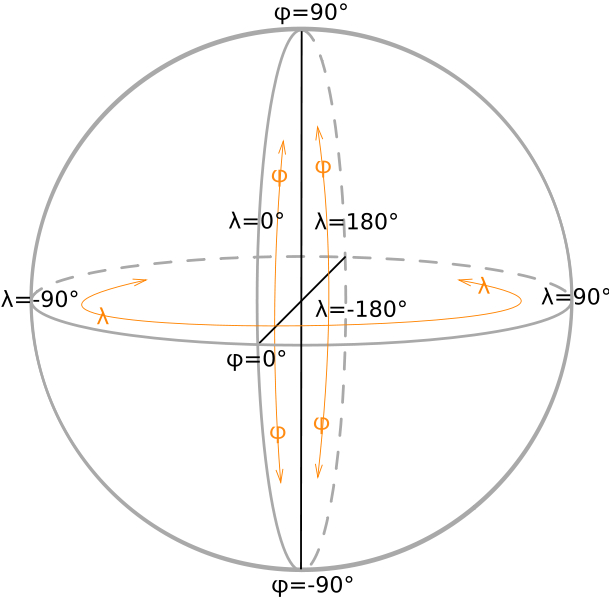
\includegraphics[width=0.4\textwidth]{./images/geographic_coordinates.jpg}              %%
	\caption[Geografische Koordinaten]{Geografische Koordinaten, Quelle: \cite{Wiki:Geo}}                        												%%
	\label{fig:geo}                                                                         %%
\end{figure}                                                                              	%%
%%%%%%%%%%%%%%%%%%%%%%%%%%%%%%%%%%%%%%%%%%%%%%%%%%%%%%%%%%%%%%%%%%%%%%%%%%%%%%%%%%%%%%%%%%%%%%
Für die Berechnung des Vektors \ensuremath{\vec{r}_{Bodenstation}} werfe man zunächst einen Blick auf das dem populären Kugelkoordinatensystem nicht ganz unähnlichen geografische Koordinatensystem (Abbildung \ref{fig:geo}). Die Koordinaten der Bodenstation im geografischen Koordinatensystem lassen sich ganz leicht ohne vor Ort zu sein mittels \href{http://www.openstreetmap.org/search?query=47.66530%2C9.44805#map=19/47.66530/9.44805}{\textit{OpenStreetMap}} herausfinden. Dabei entspricht der erste Wert dem Breiten- der zweite dem Längengrad. Der mittlere Erddurchmesser \ensuremath{d_{Erde}} beträg nach \cite{Wiki:Erde} in etwa \ensuremath{12.742 km}.
\newpar
Man stelle sich nun die Bodenstation als einen Punkt auf der Kugeloberfläche vor. Schneidet man entlang des Längengrades der Bodenstation durch die Kugel, so lässt sich mit einfacher Trigonomoetrie die Information des Breitengrades in das kartesische Koordinatensystem übetragen. Die z-Komponente des gesuchten Ortsvektors \ensuremath{\vec{r}_{Bodenstation}} ist der Sinus des Breitengrades multipliziert mit dem halben Erddurchmessser. Die Ankathete des Dreiecks, dass sich jetzt ausgebildet hat spielt bei der Betrachtung von x- und y-Komponente eine wichtige Rolle. Diese Ankathete hat die Länge des Kosinus des Breitengrads multipliziert mit dem halben Erddruchmesser. Um die x- und die y-Komponente zu ermitteln schneidet man entlang des Äquators durch die Erdkugel hindurch und wirft einen Blick auf die Schnittfläche. Die eben betonte Ankathete definiert mit der x-Achse ein weiteres rechtwinkligen Dreieck. Die Ankathete des ersten Schnitts wurde zur Hypothenuse dieses Dreiecks. Über den Längengrad und die bekannte Länge der Hypothenuse können nun x- und y-Komponente leicht bestimmt werden. Die x-Komponente folgt aus dem Kosinus des Längengrades multipliziert mit der Hypothenuse. Die y-Komponente ist eine Folge der Multiplikation des Sinus des Längengrades mit der Hypothenuse. Aus diesen einfachen und vom Kugelkoordinatensystem bekannten Denkansätzen folgt der Ortsvektor der Bodenstation. 
\begin{equation}
	\vec{r}_{Bodenstation}=\frac{d_{Erde}}{2}\,\left(\begin{array} {c}cos(latitude)\,cos(longitude)\\cos(latitude)\,sin(longitude)\\sin(latitude)\end{array}\right)
\end{equation} 
Mit diesem Vektor ist das letzte Fragment gefunden, um die Antenne über die beschriebene Vorgehensweise auszurichten und nachzufahren. Es sei darauf hingewiesen, dass die hier beschriebene Vorehensweise nicht mit einem Bahnmodell wie dem \ac{SGP4} mithalten kann. Es dient lediglich dem Verständnis. Bisher wurden auch keine Bahnstörungen berücksichtigt. Die Größte Stödas Magnetfeldrung ist dabei keine Störung der Bahn im eigentlichen Sinne, sondern die tatsache, dass die Abziehungskraft der Erde durch die Abplattung der Erde inhomogen ist. Dadurch driftet beispielsweise die Rektaszension des aufsetiegnden Knotens mit der Zeit ab.      
%\subsection{Bahnstörung}

\subsection{Bahnmodelle}
\label{chap:models}
Eines der populärsten Bahnmodelle ist das \textbf{\ac{SGP4}}. Das Bahnmodell wurde einst für das \ac{NORAD} entwickelt. Diese Institution hat u.a. die Aufgabe der Überwachung erdnaher Flugkörper. \ac{NORAD} bestimmt in regelmäßigen Zeitabständen die Bahnelemente aller katalogisierten Satelliten. Diese Informationen sind in einem bestimmten Rahmen auch zivilen Nutzern zugänglich (z.B. über \href{http://celestrak.com/}{\textit{Celestrak}}). Hiervon profitieren eben solche Amateurfunk-Bodenstationen wie die der DHBW Friedrichshafen. Die Distribution der \ac{NORAD}-Bahnelemente „erfolgt in einem zweizeiligen Datenformat, was zu dem Beinamen \ac{TLE} geführt hat“ (siehe S. 95 in \cite{HandRaum}). Das Format der \ac{TLE} ist in Abbildung \ref{fig:tle} gut beschrieben. Es ist zu beachten, dass es sich bei den Bahnelementen, welche von \ac{NORAD} geliefert werden um mittlere Bahnelemente handelt. Diese sind im Gegensatz zu den tatsächlichen (oskulierenden) Bahnelementen nicht für eine Auswertung mit dem oben beschriebenen Keplerschen Bahnmodell verwendbar, sondern nur für die Verwendung in dem analytischen Modell mit welchem sie generiert wurden verwertbar. 
%%%%%%%%%%%%%%%%%%%%%%%%%%%%%%%%%%%%%%%%%%%%%%%%%%%%%%%%%%%%%%%%%%%%%%%%%%%%%%%%%%%%%%%%%%%%%%
\begin{figure}[h]                                                                           %%
	\centering                                                                            	%%
	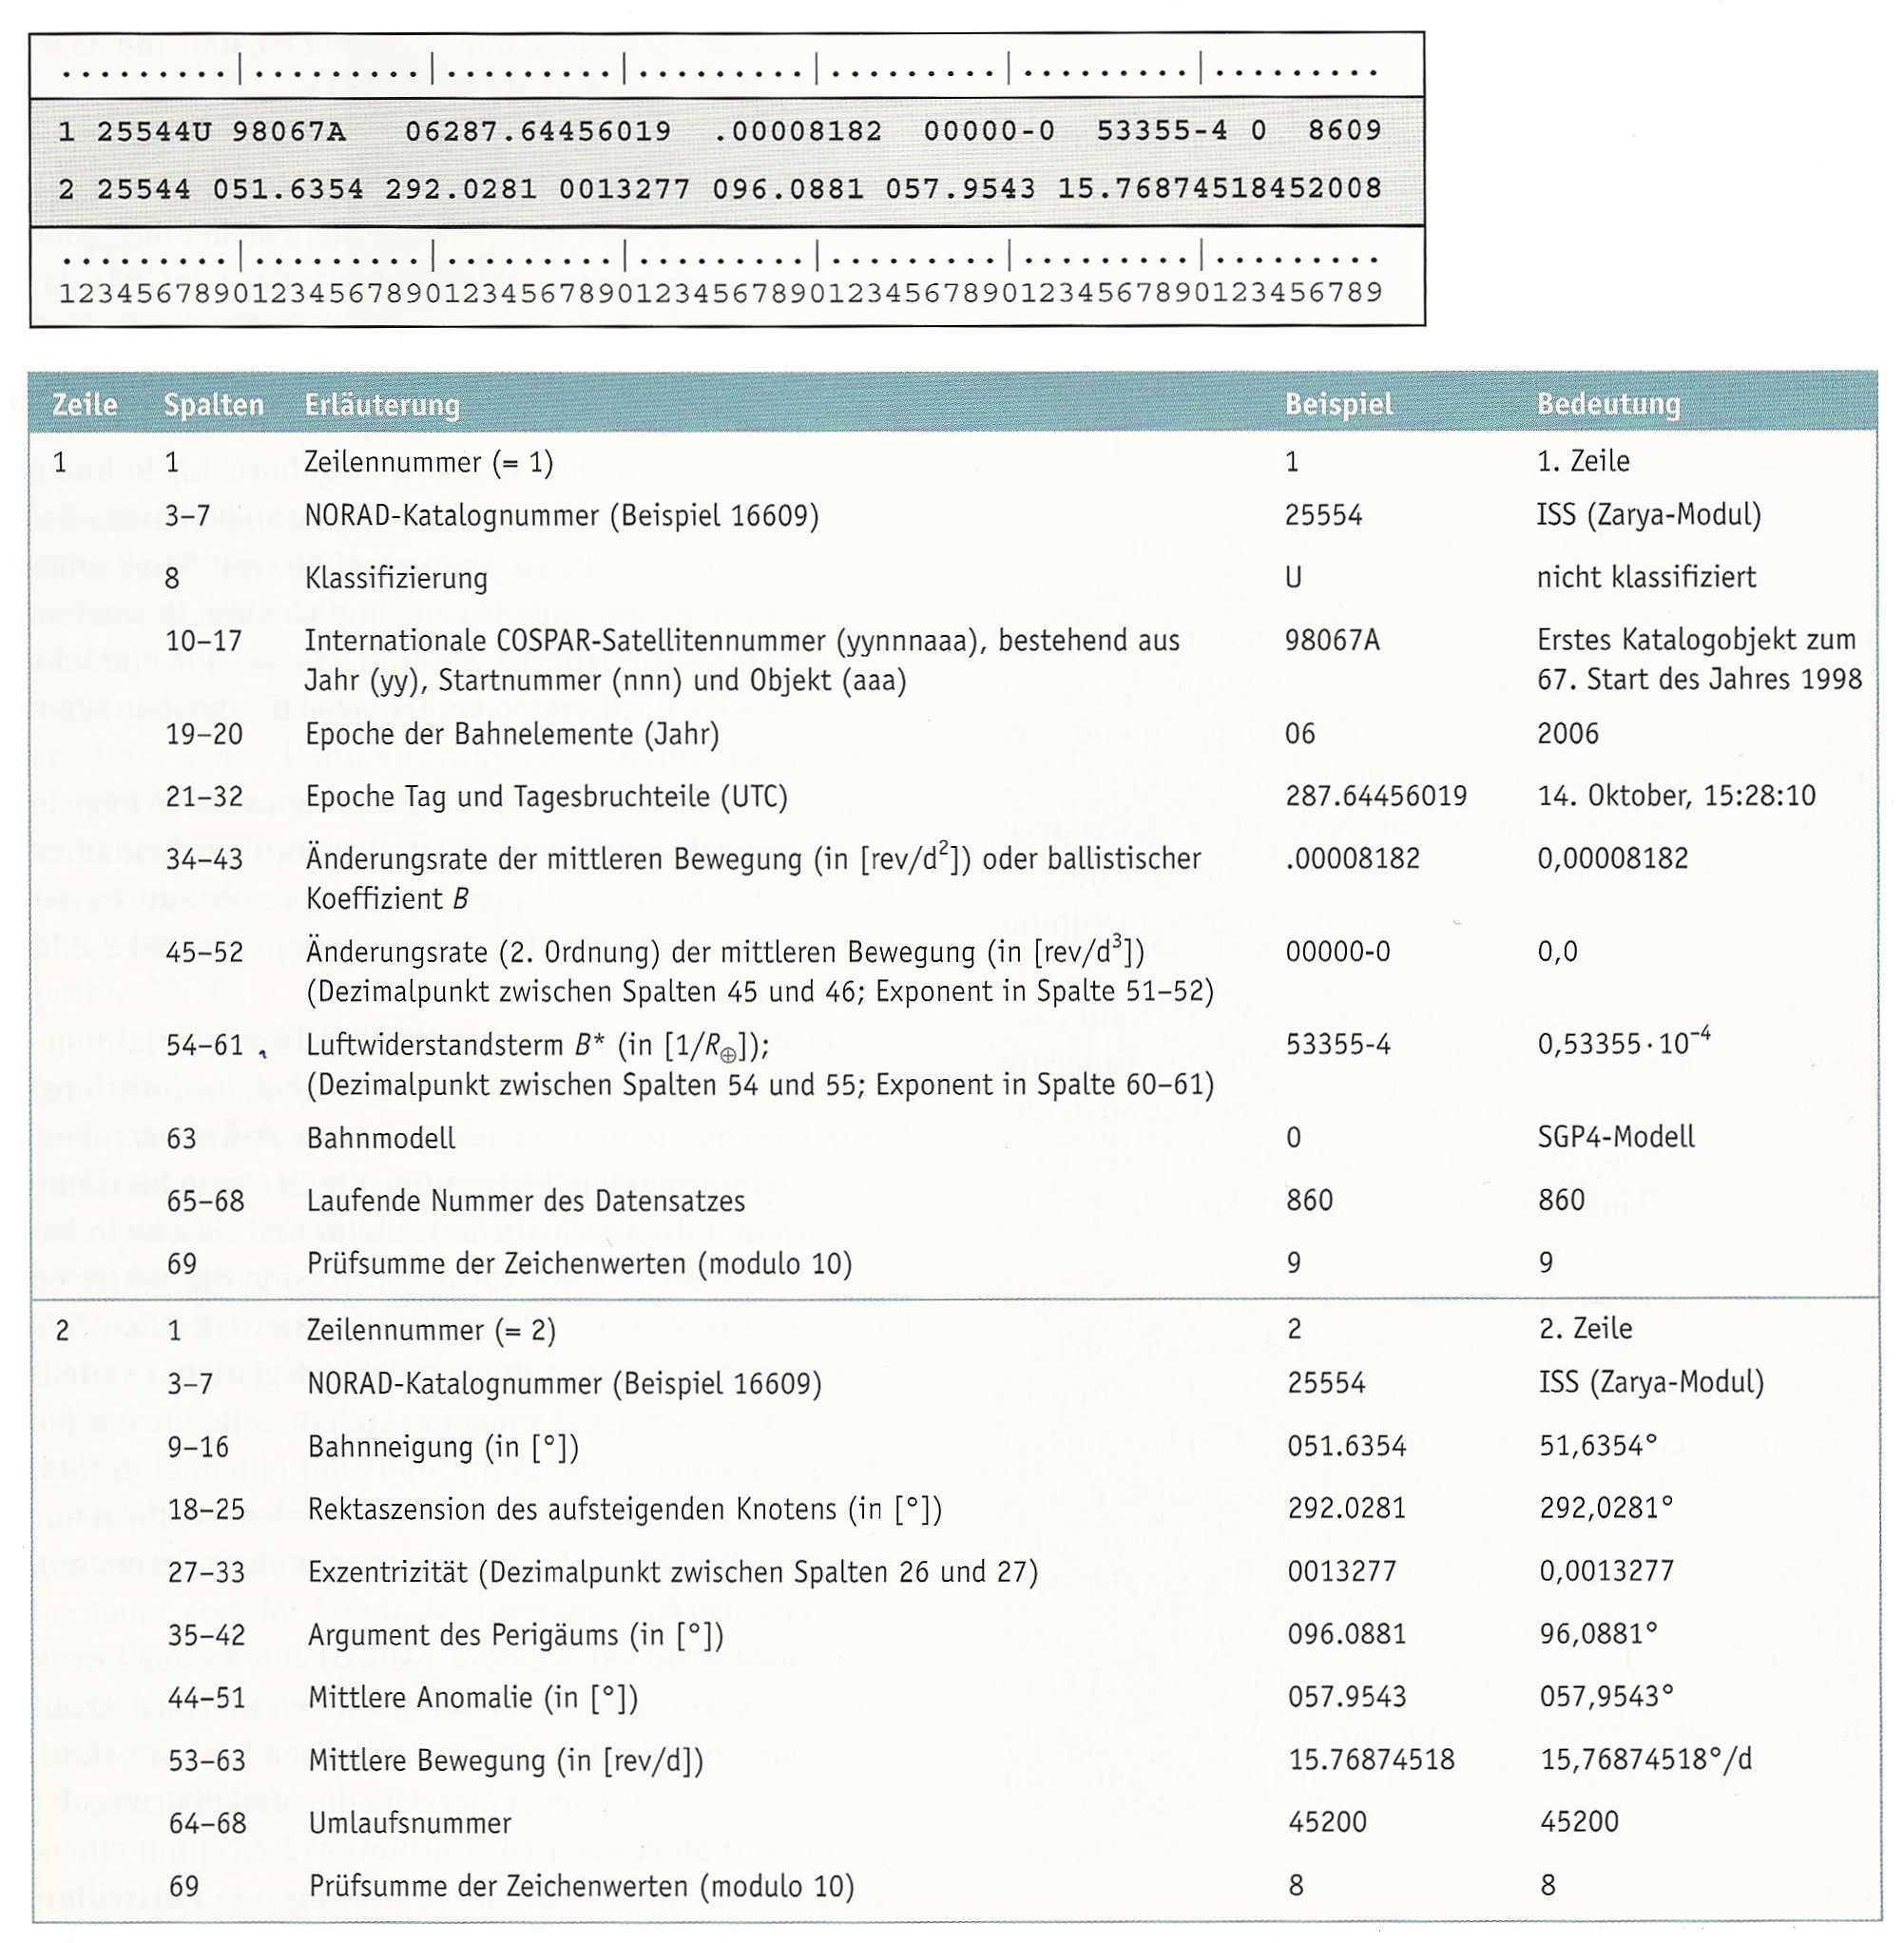
\includegraphics[width=0.96\textwidth]{./images/tle.jpg}              			            %%
	\caption[\ac{TLE}]{\ac{TLE}, Quelle: S.96 in \cite{HandRaum}}                           %%
	\label{fig:tle}                                                                         %%
\end{figure}                                                                              	%%
%%%%%%%%%%%%%%%%%%%%%%%%%%%%%%%%%%%%%%%%%%%%%%%%%%%%%%%%%%%%%%%%%%%%%%%%%%%%%%%%%%%%%%%%%%%%%%   
Das \ac{SGP4} entstand um 1970 und basiert auf einem analytischen Model von Lane und Crawford. Deren Modell verband zu deren Zeit die gravitativen Störungen mit einem analytischen Modell zur Beschreibung des Luftwiderstands. Für den operationellen Einsatz haben Lane und Hoots die vollständige Theorie vereinfacht und so in da \ac{SGP4} überführt. 
\newpar
Außer dem \ac{SGP4} verwendet  GPredict auch das \ac{SDP4}. „Es erfasst zusätzlich Störungen durch die Gravitationskraft von Sonne und Mond, sowie [Informationen], die bei Bahnen mit einer Umlaufzeit von 12 h (GPS) und 24 h ([bei ]geostationäre[n] Satelliten) von Bedeutung sind“ (siehe S. 96 in \cite{HandRaum}). Das \ac{SDP4} kommt bei Satelliten mit einer Umlaufzeit von mehr als 225 Minuten zum Zug. Derartige Satelliten bewegen sich auf sog. „Deep Space“-Bahnen. 
\newpar
Aus Abbildung \ref{fig:sgp4} ist ein Gefühl für die Genauigkeit des \ac{SGP4} entnehmbar. Nahe an der Epoche liegt die Abweichung im Bereich von wenigen Kilometern. Die Abweichung kommt von mehreren kurzperiodischen Störungen, die das Bahnmodell unterschlägt. Innerhalb von mehreren Tagen nimmt die Abweichung mit quadratischer Abhängigkeit zu. Laut \cite{HandRaum} ist der Grund dieses Fehlers die nicht vorhersagbare Atmosphärendichte. Bei höhren Flugbahnen sind die Fehler deswegen allgemein deutlich kleiner. Eine ziehmlich genaue Bahnprediktion über mehrere Wochen ist so,it nicht unrealistisch. Als Fazit lässt sich sagen, dass die Bahnelemente mit den GPredict arbeitet regelmäßig aktualisiert werden sollten, um eine optimale Leistungsfähigkeit der Bodenstation zu erreichen.  
%%%%%%%%%%%%%%%%%%%%%%%%%%%%%%%%%%%%%%%%%%%%%%%%%%%%%%%%%%%%%%%%%%%%%%%%%%%%%%%%%%%%%%%%%%%%%%
\begin{figure}[h]                                                                           %%
	\centering                                                                            	%%
	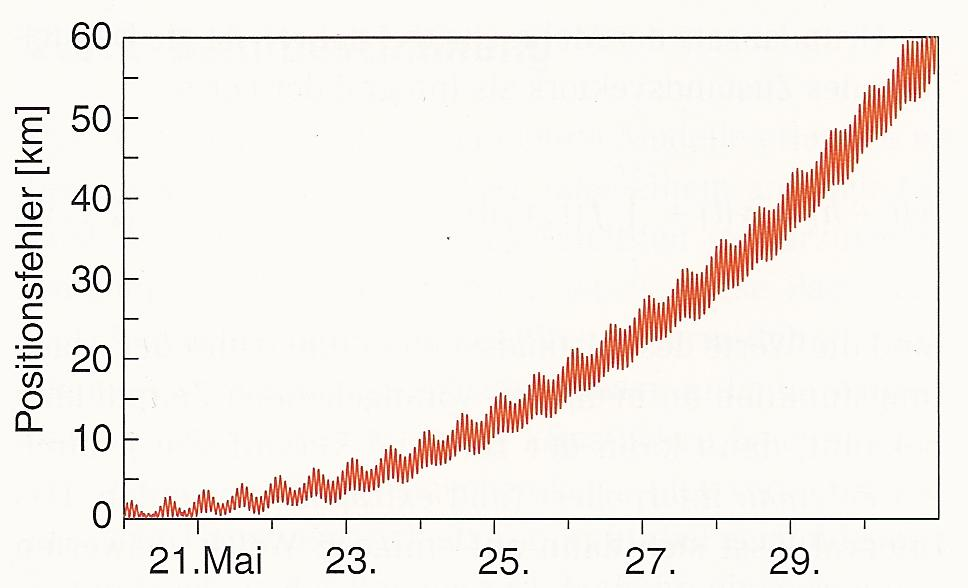
\includegraphics[width=0.6\textwidth]{./images/sgp4_error.jpg}              			%%
	\caption[Vorhersagegenauigkeit]{Vorhersagegenauigkeit des Satelliten CHAMP 
	im Mai 2001, Quelle: S.96 in \cite{HandRaum}}                        					%%
	\label{fig:sgp4}                                                                        %%
\end{figure}                                                                              	%%
%%%%%%%%%%%%%%%%%%%%%%%%%%%%%%%%%%%%%%%%%%%%%%%%%%%%%%%%%%%%%%%%%%%%%%%%%%%%%%%%%%%%%%%%%%%%%% 

\subsection{Der Doppler-Effekt}
Der folgende Abschnitt entstammt einer Seminararbeit der Autoren eben dieser Arbeit vom 16. November 2015 aus der Vorlesung Radartechnik von Jürgen Göbel. 

Ein Beobachter, der sich relativ zu einem Wellensender bewegt, registriert 
eine andere Frequenz als die von der Quelle gesendete Frequenz. Bei der 
Näherung von Sender und Empfänger scheint die Frequenz erhöht und bei einer 
Entfernung verkleinert. Dieses Phänomen wurde 1842 von C.J.Doppler entdeckt. 

\subsubsection{Der Doppler-Effekt in der Akustik}
Wollen wir die Wellenlänge oder die Frequenz berechnen, müssen wir 
unterscheiden, ob die Quelle sich bewegt und der Empfänger ruht oder ob sich 
der Empfänger bewegt und die Quelle ruht.\\
\textbf {1. Bewegte Quelle und ruhender Empfänger:}\\
Eine Quelle bewegt sich mit einer Geschwindigkeit und sendet Wellen mit einer 
Wellenlänge aus, die sich mit der Lichtgeschwindigkeit ausbreiten.  
Nun nähert sich die Wellenfront auf den Empfänger zu. 
Er registriert eine verkleinerte Wellenlänge, als die ausgesandte.\\
\textbf {2. Bewegter Empfänger und ruhende Quelle:}\\
Bewegt sich der Empfänger und ruht die Quelle, ändert sich die Wellenlänge 
nicht, jedoch die Frequenz vom  Empfänger registrierten Wellen. 
Bewegt sich der Empfänger zu der ruhenden Quelle, ist die Frequenz erhöht 
und wendet es sich ab, ist sie verringert. Ruht der Empfänger, treffen ihn die 
Wellen die auf der Strecke zu finden sind. 
Bewegt er sich zu der Quelle, kommen zusätzlich Wellenzüge von hinzu. \\
Die Beschreibung entspricht weitgehend derjenigen bei elektromagnetischen 
Wellen mit einer Ausnahme:\\ 
\textbf{Das Licht benötigt kein Medium um sich auszubreiten und breitet sich 
	immer gleich schnell aus, unabhängig von dem Bewegungszustand der Lichtquelle}
(Postulat von der Konstanz der Vakuumlichtgeschwindigkeit c, Albert Einstein 
1905).

\subsubsection{Physikalische Hintergründe und Herleitung}
Um ein grundlegendes  physikalisches Verständnis für den Doppler-Effekt zu entwickeln, 
gehe man zunächst von einem akustischen Beispiel aus dem Alltag aus: Ein Rennwagen fahre auf einem Beobachter 
mit der Geschwindigkeit \begin{math}v_R=70 \frac{m}{s}\end{math} zu. Der Beobachter habe dabei 
keine Eigengeschwindigkeit \begin{math}v_B=0 \end{math} relativ zum Bezugsystem Rennstrecke. Im 
Spektrum des vom Auto emittierten akustischen Signals sei ein Sinussignal der Frequenz \begin{math}f_R=1kHz\end{math} 
enthalten. Aus Sicht des Rennwagenfahrers hat das emittierte Signal die Wellenlänge
\begin{math}\lambda_R=\frac{c_S}{f_R}=\frac{340\frac{m}{s}}{1kHz}=0,34m\end{math}.
Aus Sicht des Beobachters sieht das Ganze etwas anders aus. 
Man nehme an, der Rennwagen emittiere zunächst einen Wellenberg.
Bis der zweite Wellenberg emittiert wird ist der Rennwagen allerdings schon ein Stück \begin{math}\delta s_R\end{math} auf den Beobachter zu gefahren. Diese Bewegung relativ
zum Beobachter hat zur Folge, dass sich die Wellenlänge um genau dieses Stück verkürzt bzw. verlängert, wenn der Rennwagen sich vom Beobachter fortbewegt.
Die Wellenlänge aus Sicht des Beobachters ist nun wie folgt zu beschreiben.
\begin{equation}
\label{lambda_b}
\lambda_B=\lambda_R -\delta s_{R}=\lambda_R - v_R \cdot T_{R}=\lambda_R - \frac{v_R}{f_{R}}
\end{equation} 
Mit den gegebenen Werten ergibt sich eine neue Wellenlänge \begin{math}{\lambda_B=0,27m} \end{math}. Da \begin{math}{\lambda_B \sim \frac{1}{f_B}} \end{math}  
ergibt sich auch eine neue Frequenz von \begin{math}{f_B \approx 1260 Hz} \end{math}. Nun geht man noch ein Stück weiter, so dass man eine Funktion 
\begin{math}{f_B(f_R,v_R)} \end{math} erhält. Hierzu wird Gleichung \ref{lambda_b} herangezogen. Es muss nur noch die Beziehung \begin{math}{\lambda=\frac{c_S}{f}} \end{math} 
einmal für die Wellenlänge des Rennwagens und einmal für die Wellenlänge des Beobachters eingesetzt werden. Dann ist die Gleichung nach \begin{math}{f_B} \end{math} aufzulösen.  
Das Ergebnis ist dann         
\begin{equation}
\label{freq_b}
f_B=\frac{f_R}{1-\frac{v_R}{c_S}}
\end{equation}
Entfernt sich der Rennwagen ist für die Geschwindigkeit des selbigen einfach ein negativer Wert einzusetzen. \textbf{Achtung:} Soll der Doppler-Effekt auf eine sich in einem Medium fortbewegende
Welle angewandt werden, ist von den Gleichungen her immer zwischen bewegtem Sender, bewegtem Empfänger und bewegtem Sender, sowie bewegtem Empfänger zu unterscheiden. 
Die oben aufgeführten Gleichungen beziehen sich ausschließlich auf den Fall, dass sich der Sender bewegt. 
\\Elektromagnetische Wellen brauchen wie seit dem 20 Jahrhundert allgemein bekannt kein Medium, um sich fortzupflanzen. Bewegen sich Sender oder Empfänger relativ zueinander, so kommt es auch bei elektromagnetischen Wellen zum Dopplereffekt. Aufgrund dessen, dass die Ausbreitung nicht auf das Medium angewiesen ist, spielt es keine Rolle, ob sich Empfänger, Sender oder beide bewegen. Die Frequenzverschiebung ist nur noch von der Relativgeschwindigkeit abhängig. Das Relativitätsprinzip besagt nun, dass sich jeder Übertragungsteilnehmer als ruhend betrachten darf. (Aus physikalischer Sicht kann man tatsächlich behaupten, dass jemand einem vor der Diskothek "`in die Faust gelaufen"' ist). Dank diesen Prinzips ist der obige akustische Fall (siehe Gleichung \ref{freq_b}) universell direkt auf eine Übertragung mit elektromagnetischen Wellen umsetzbar. 
\\Das ist allerdings nur die halbe Wahrheit. Es gibt leider keine absolute Zeit. Die Gleichzeitigkeit von räumlich getrennten Ereignissen ist eine Frage der Relativgeschwindigkeit des Beobachters. 
\\Der relativistische Effekt der Zeitdillitation ist beim Doppler-Effekt mitzubetrachten, da die Periodendauer des emittierten Signals aus Sicht des Beobachters auf der Erde aufgedehnt wird. Somit wird die Wellenlänge des Sendesignals \begin{math}{\lambda_S}\end{math} größer und die Frequenz des selbigen \begin{math}{f_S}\end{math} kleiner. Mit dieser Erkenntnis folgt nun die tatsächliche Gleichung für den Dopplereffekt.  
\begin{equation}
\label{freq_e1}
f_E=\frac{f_S}{1-\frac{v_r}{c_L}}\cdot \frac{1}{\gamma}=\frac{f_S\sqrt{1-\left(\frac{v}{c_L}\right)^2}}{1-\frac{v_r}{c_L}}
\end{equation} 
Hierbei ist \begin{math}{f_E}\end{math} die vom Empfänger empfangene Frequenz, \begin{math}{v_r}\end{math} die radiale Relativgeschwindigkeit von Sender und Empfänger und \begin{math}{c_L}\end{math} die Lichtgeschwindigkeit. Die tangentialen Anteile der Bewegung interessieren den Beobachter im nicht relativistischen Teil der Gleichung natürlich nicht. Es sind nur die radialen Anteile für den Doppler-Effekt relevant. Filtert man also den tangentialen Anteil mittels des Kosinus aus der Relativgeschwindigkeit aus, so kann man für die Geschwindigkeit einfach die betragsmäßige Relativgeschwindigkeit einsetzen.   
\begin{equation}
\label{freq_e2}
f_E=\frac{f_S\sqrt{1-\left(\frac{v}{c_L}\right)^2}}{1-\frac{v}{c_L} \cdot cos(\alpha)}
\end{equation}
Bewegt sich nun der Sender rein tangential zum Empfänger würde man keinen Doppler-Effekt erwarten. Aufgrund der Relativgeschwindigkeit von Sender und Empfänger tritt jedoch die Zeitdillitation nach wie vor auf. Man spricht in diesem Fall vom transversalen Doppler-Effekt.    

% Software
%%%%%%%%%%%%%%%%%%%%%%%%%%%%%%%%%%%%%%%%%%%%%%%%%%%%%%%%%%%%%%%%%%%%%%%%%%%%%%%%%%
%%																				%%
%% File name: 		20hannes.tex												%%
%% Project name:	Hochleistungsantenne										%%
%% Type of work:	T3X00 project work											%%
%% Author:			Sarah Brückner, Maximilian Stiefel, Hannes Bohnengel		%%
%% Date:			14th May 2016												%%
%% University:		DHBW Ravensburg Campus Friedrichshafen						%%
%% Comments:		Created in gedit with tab width = 4							%%
%%																				%%
%%%%%%%%%%%%%%%%%%%%%%%%%%%%%%%%%%%%%%%%%%%%%%%%%%%%%%%%%%%%%%%%%%%%%%%%%%%%%%%%%%

\chapter{GPredict}

\section{Übersicht}

GPredict ist eine freie Software zur Satellitenverfolgung und Orbitvorhersage und steht als Quellcode oder bereits fertig kompiliertes Programm für Windows, Mac OS und Linux zur Verfügung. Die Software ist in C geschrieben und unter der GNU \ac{GPL} lizenziert, somit kann sie frei verändert und an die entsprechenden Nutzervoraussetzungen angepasst werden.\newpar
In Abbildung \ref{fig:gpredict-principle} ist das Prinzip eines Satellitenverfolgungsprogramms zu sehen (die blauen Blöcke stellen hierbei die Funktionalität des Programms dar). Zunächst wird an Hand der Keplerschen Bahnelemente und dem aktuellen Zeitpunkt die absolute Position des Satelliten berechnet. Daraufhin wird der Vektor, der von der Bodenstation zum Satelliten zeigt, bestimmt. Nun können Azimut und Elevation dieses Vektors für die Ansteuerung der Antenne verwendet werden.

\begin{figure}[h]
	\centering
	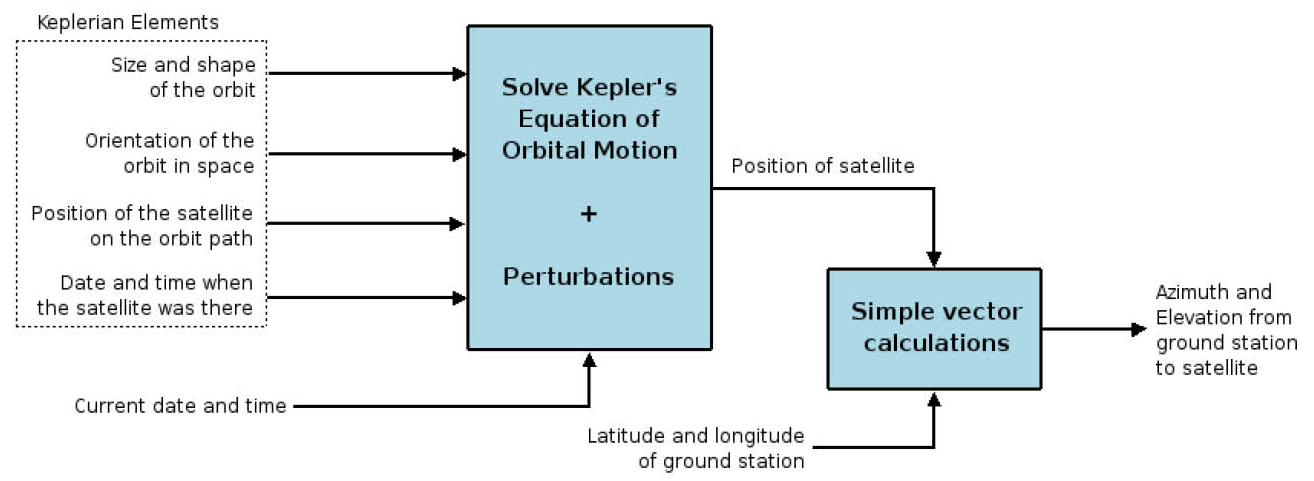
\includegraphics[width=1\textwidth]{gpredict-principle}
	\caption{Prinzip eines Satellitenverfolgungsprogramms \cite{gpredictmanual}}
	\label{fig:gpredict-principle} 
\end{figure}

Zur Berechnung der Satellitenposition wird auf den NORAD SGP4/SDP4 Algorithmus zurückgegriffen (siehe Abschnitt XXX). Um hierfür zu jedem Zeitpunkt die aktuellen Kepler-Elemente des zu verfolgenden Satelliten zu kennen, gibt es unter GPredict die Möglichkeit einer automatischen Aktualisierung über HTTP, FTP oder aus dem lokalen Verzeichnis.

\clearpage

Bei GPredict ist im Gegensatz zu anderen Satellitenverfolgungsprogrammen wie SatPC32 kein Limit an zu verfolgenden Satelliten und Bodenstationen gegeben. Durch die Verwendung von Modulen kann außerdem unkompliziert zwischen verschiedenen Konfigurationen gewechselt werden. Die Orbitvorhersage eines Satelliten lässt sich sowohl grafisch als auch tabellarisch darstellen, wobei durch die Einstellungen verschiedenster Parameter eine sehr individuelle Anzeige erreicht werden kann \cite{gpredictsource}.

\section{Grafische Oberfläche}

In Abbildung \ref{fig:gpredictstartup} ist die grafische Oberfläche von GPredict zu sehen. In der Standardkonfiguration ist dort zunächst die Kartenansicht bzw. \myemph{Map View} (oben), die Polaransicht bwz. \myemph{Polar View} (links unten) und die Einzelsatellitenansicht bzw. \myemph{Single-Satellite View} (rechts unten) zu sehen.

\begin{figure}[h]
	\centering
	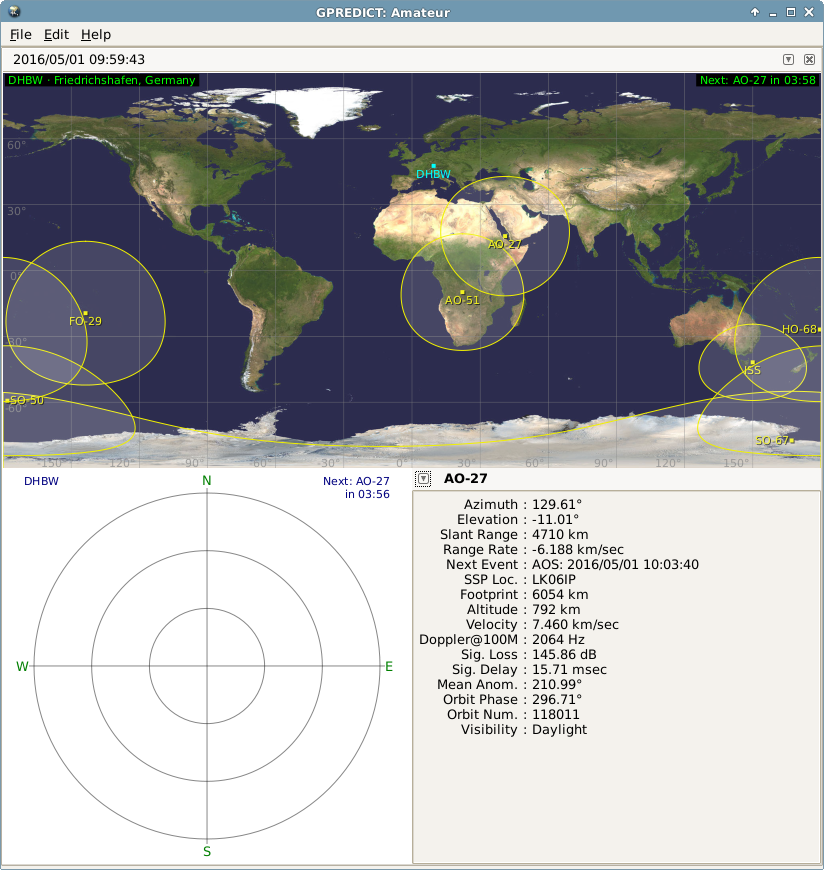
\includegraphics[width=0.75\textwidth]{gpredict-startup}
	\caption{Standardoberfläche von GPredict}
	\label{fig:gpredictstartup} 
\end{figure}

\clearpage

\subsection{Grundansichten}

Zu den oben genannten Ansichten kommen noch zwei Weitere hinzu, die Listenansicht bzw. \myemph{List View} und eine Ansicht für bevorstehende Vorbeiflüge, die sogenannte \myemph{Upcoming Passes View}. Im Folgenden werden die verschiedenen Ansichten genauer beschrieben:\newpar
\textbf{Map View}\\
Diese Ansicht besteht, wie in Abbildung \ref{fig:gpredictstartup} zu sehen, aus einer Weltkarte auf der die aktuellen Standorte der für das aktuelle Modul ausgewählten Satelliten zu sehen ist. Das heißt der Punkt auf dem der entsprechende Satellit senkrecht bezogen auf den Erdmittelpunkt steht. Außerdem ist um diesen Punkt die Fläche umrahmt, von der der Satellit von der Erde aus sichtbar ist. Mit einem Rechtsklick auf einen Satellitennamen kann außerdem die Option \myemph{Ground Track} aktiviert werden, mit welcher die Spur des Satelliten für mehrere Orbits angezeigt wird.\newpar
\textbf{Polar View}\\
Die \myemph{Polar View} (siehe Abbildung \ref{fig:gpredictstartup}) stellt eine Draufsicht auf die Bodenstation dar, bei der die Polarachse den Azimutwinkel darstellt und die Radialachse den Elevationswinkel. Mit einem Rechtsklick auf einen Satelliten lässt sich mit der Option \myemph{Show sky track} aktivieren, das die Spur des entsprechenden Satelliten anzeigt wird. Zusätzlich wird das aktuelle Modul links oben angezeigt, der nächste sichtbare Satellit (rechts oben) und die genauen Werte für Azimut und Elevation (links unten) sobald sich der Mauszeiger auf der \myemph{Polar View} befindet.\newpar
\textbf{Single-Satellite View}\\
In dieser Ansicht (siehe Abbildung \ref{fig:gpredictstartup}) werden detaillierte Informationen zu einem ausgewählten Satelliten angezeigt, z.B. Azimut, Elevation, Entfernung der direkten Sichtverbindung (\myemph{Slant Range}), Höhe, Geschwindigkeit, Dopplerverschiebung oder Signaldämpfung. Mit einem Klick auf das Dreieck links neben dem Satellitennamen kann zwischen den für dieses Modul ausgewählten Satelliten gewechselt werden.

\clearpage

\textbf{List View}\\
Die Listenansicht zeigt eine tabellarische Auflistung aller für das aktuelle Modul ausgewählten Satelliten mit verschiedenen Details, mit je einem Satelliten pro Zeile. In Abbildung \ref{fig:listview} ist die Listenansicht mit allen verfügbaren Details zu sehen. Mit einem Klick auf eine entsprechende Kategorie lässt sich das Sortierkriterium ändern. Falls hier ein variables Kriterium wie die Geschwindigkeit eingestellt wird, ändert sich die Sortierreihenfolge mit der eingestellten Auffrischrate (\myemph{Refresh Rate}). Die Bezeichnung des jeweiligen Details ist in dieser Ansicht abgekürzt, z.B. \myemph{Az} für \myemph{Azimut}. Unter den Moduleinstellungen beim Reiter \myemph{List View} kann ausgewählt werden, welches Detail angezeigt wird. Dort ist außerdem erkenntlich für was die entsprechenden Abkürzungen stehen.

\begin{figure}[h]
	\centering
	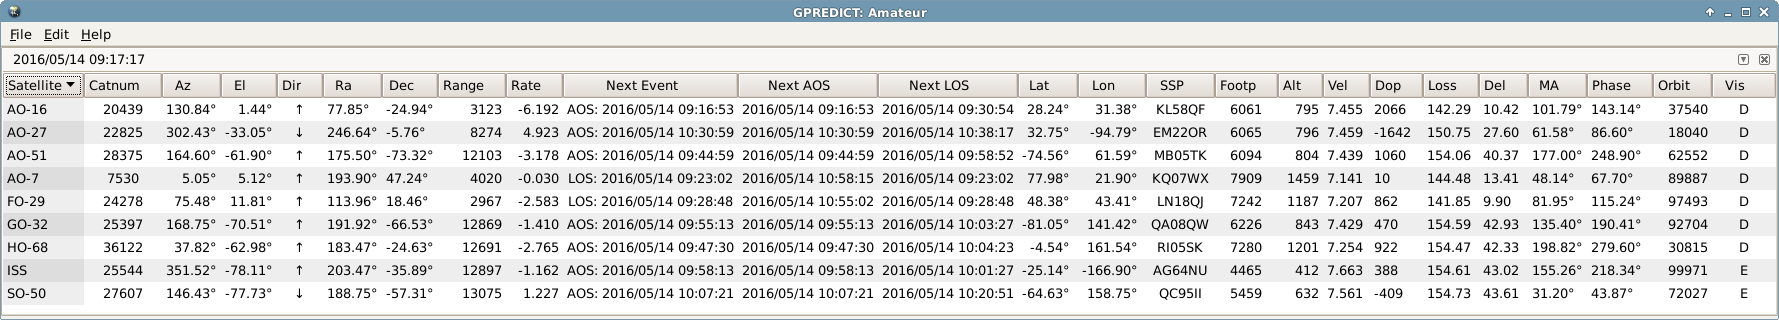
\includegraphics[width=1\textwidth]{listview}
	\caption{Listenansicht bzw. \myemph{List View} von GPredict}
	\label{fig:listview} 
\end{figure}

\textbf{Upcoming Passes View}\\
Die \myemph{Upcoming Passes View} (siehe Abbildung \ref{fig:upcomingpassesview}) zeigt alle Satelliten des aktuellen Moduls, deren Azimut und Elevation, sowie die Zeit bis zum nächsten Verschwinden des Satelliten, dem sogenannten \myemph{\ac{LOS}} bzw. dem nächsten Auftauchen, auch \myemph{\ac{AOS}} genannt.

\begin{figure}[h]
	\centering
	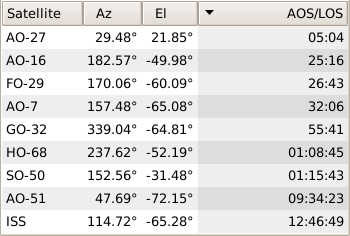
\includegraphics[width=0.3\textwidth]{upcomingpassesview}
	\caption{Upcoming Passes View}
	\label{fig:upcomingpassesview} 
\end{figure}

\clearpage

\subsection{Weitere Ansichten}

Bei allen Ansichten kann durch einen Klick auf den Satellitennamen (bei der \myemph{Single-Satellite View} ein Klick auf das Dreieck neben dem Namen) ein kleines Pop-Up Menü geöffnet werden, welches den entsprechenden Satellitennamen, die Option \myemph{Show next pass} und die Option \myemph{Future passes} anzeigt.

\begin{figure}[h]
	\centering
	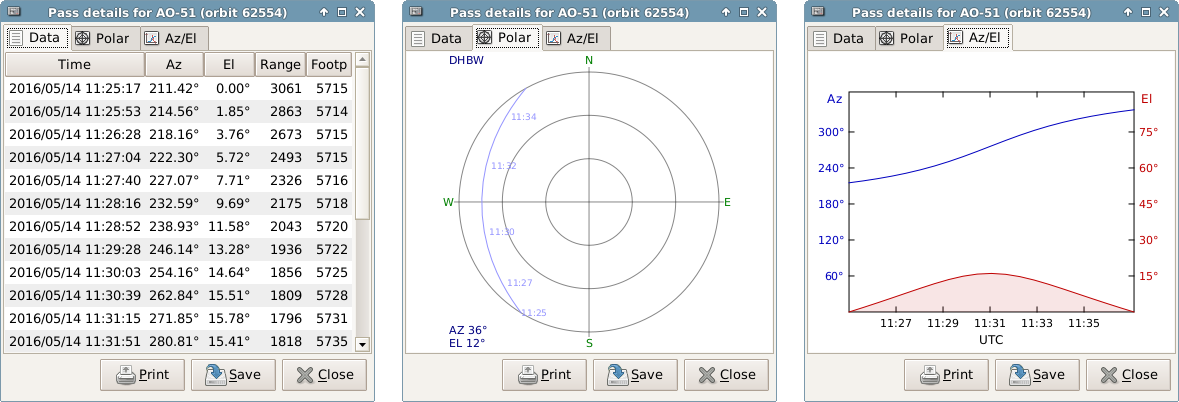
\includegraphics[width=1\textwidth]{passdetails}
	\caption{Pass Details}
	\label{fig:passdetails} 
\end{figure}

\begin{figure}[h]
	\centering
	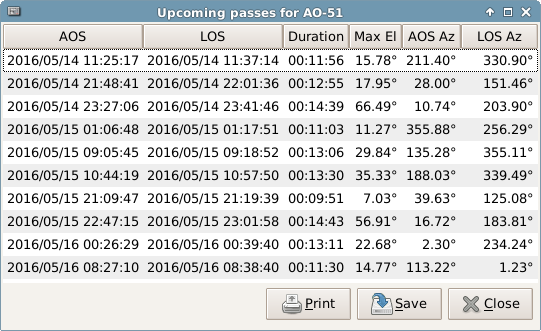
\includegraphics[width=0.5\textwidth]{upcomingpasses}
	\caption{Upcoming Passes}
	\label{fig:upcomingpasses} 
\end{figure}

\begin{figure}[h]
	\centering
	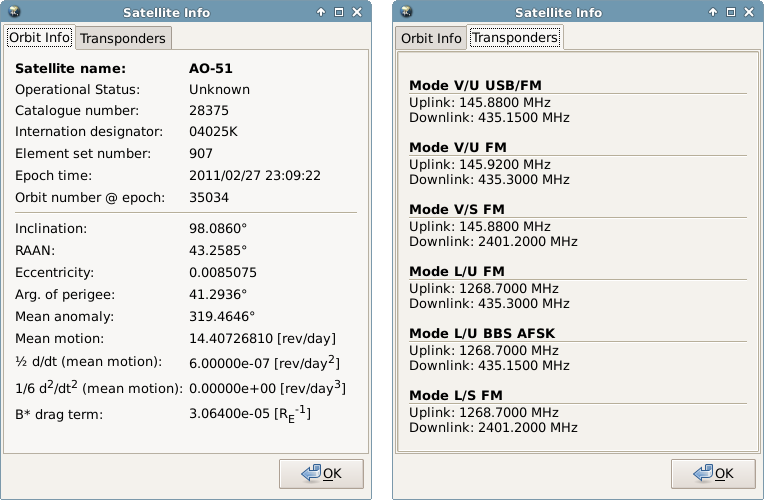
\includegraphics[width=0.7\textwidth]{satinfo}
	\caption{Satellite Info}
	\label{fig:satinfo} 
\end{figure}

\clearpage

\subsection{Modul Pop-Up Menü}

\begin{itemize}
	\parskip0pt
	\item \textbf{Antenna Control (Rotoren):} (noch kein Bild vorhanden)
	\item \textbf{Radio Control} (noch kein Bild vorhanden)
	\item \textbf{Sky at a Glance} (theskyataglance.png)
	\item \textbf{Time Controller} (timecontroller.png)
	\item \textbf{Modul-Einstellungen} (editmodule.png)
\end{itemize}

\subsection{GPredict Einstellungen}

\begin{itemize}
	\parskip0pt
	\item \textbf{General}
	\item \textbf{Modules}
	\item \textbf{Interfaces}
	\item \textbf{Predict}
\end{itemize}


\iffalse
\textbf{Map View}\\
alskfjlöajsf aöfljasldkfj laksjf lkad fasd\newpar
\textbf{Polar View}\\
öasjf lasj lkösda fj lfk kajj dj lk fas 
\fi

\clearpage

\section{HamLib-Programmierschnittstelle}

\begin{figure}[h]
	\centering
	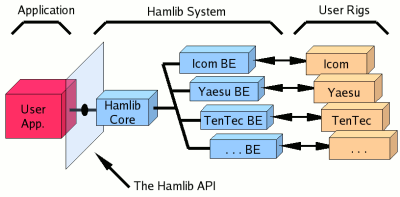
\includegraphics[width=0.5\textwidth]{hamlib}
	\caption{HamLib Design \cite{hamlib}}
	\label{fig:hamlib} 
\end{figure}

\section{Inbetriebnahme unter Windows}

Dieser Text soll ein Test sein, ob die .tex File auch online bearbeitet werden kann.

\section{Inbetriebnahme unter Linux}


%---- Conclusion -----------------------------------------------------------------

%%%%%%%%%%%%%%%%%%%%%%%%%%%%%%%%%%%%%%%%%%%%%%%%%%%%%%%%%%%%%%%%%%%%%%%%%%%%%%%%%%
%%																				%%
%% File name: 		conclusion.tex												%%
%% Project name:	Hochleistungsantenne										%%
%% Type of work:	T3X00 project work											%%
%% Author:			Sarah Brückner, Maximilian Stiefel, Hannes Bohnengel		%%    
%% Date:			01st May 2016											    %%
%% University:		DHBW Ravensburg Campus Friedrichshafen						%%
%% Comments:		Created in gedit with tab width = 4							%%
%%																				%%
%%%%%%%%%%%%%%%%%%%%%%%%%%%%%%%%%%%%%%%%%%%%%%%%%%%%%%%%%%%%%%%%%%%%%%%%%%%%%%%%%%

\chapter{Zusammenfassung und Ausblick}
Im Verlauf dieser Studienarbeit "`Inbetriebnahme einer freien Software zur Satellitenbahnvorhersage und Ansteuerung einer Hochleistungsantenne"' wurde eine freie Software validiert und in Betrieb genommen. Zusammenfassend kann man sagen, dass die Studiearbeit nach umfangreichen Tests zu dem Ergebnis kam, dass die freie Software GPredict eine sehr gute Alternative zu der Referenzsoftware SatPC32 ist. 
\newpar
GPredict ist ein Satelliten-Tracking Programm und ermöglicht eine Anbindung an die Antennenrotoren sowie 
an das Funkgerät. Unter der Verwendung der \ac{TLE} berechnet GPredict die jeweilige Satellitenbahn und veranschaulicht diese mit einer Vielzahl an Extras in der grafischen Oberfläche des Programms. Um grob verstehen zu können, wie GPredict eine Bahnvorhersage durchführt und was sich physikalisch dahinter verbirgt, wurden die physikalischen Hintergründe in möglichst kompakter auf das Thema zugeschnittener Weise aufbereitet. Dieses physikalische Verständnis ist notwendig, damit man als an der Bodenstation arbeitender Wissenschaftler "`weiss was man tut"'. Eine auf dieser Studienarbeit aufbauenden wissenschaftlichen Arbeit muss somit wichtige Grundlagenrecherchen zum Kepler-Problem etc. nicht mehr abhandeln. Für die an der Arbeit des Aufbaus der Bodenstation involvierten Wissenschaftler bietet die Ihnen vorliegende Studienarbeit einen schnellen Einstieg.     
\newpar
Um GPredict an die Hardwareumgebung anzubinden, wurde eine entsprechende Konfiguration von GPredict vorgenommen. Die Funkgerätansteuerung und Antennenausrichtung erfolgt mittels der Hamlib--Bibliothek. Dafür wurden eigene Batch-Skripte geschrieben um die Verwendung der verfügbaren Kommandozeilenprogramme zu vereinfachen. 
\newpar
Für die Validierung der Anforderungsdefinition, wurden vorher festgelegte Tests durchgeführt. Dabei handelte es sich um Modultests, Integrationstests und Systemtests. 
\newpar
Als Fazit ist festzuhalten, dass die Studienarbeit gemäß dem V-Modell bearbeitet und strukturiert wurde. Das Ergebnis der Studienarbeit korreliert mit der Anforderungsdefinition und bietet eine Grundlage für weitere Studienarbeiten an der Bodenstation der DHBW Ravensburg Campus Friedrichshafen. Dabei wäre eine weitere Aufgabe die Implementierung eines Befehls zum Tausch von Sub-- und Main--Band.
\newpar
Im Rahmen dieser Studienarbeit wurden die Inhalte der Nachrichtentechnik und des technischen Managements reflektiert und aus Sicht von Nachrcihtentechnikern ein neues Gebiet der Bahnmechanik erschlossen. 
\clearpage


%---- vvv ROMAN PAGE NUMBERING vvv -----------------------------------------------

\pagenumbering{Roman}
\setcounter{page}{\value{romanPagenumber}}

%---- List of figures ------------------------------------------------------------

\listoffigures
Alle hier nicht eigens nachgewiesenen Abbildungen stammen vom Autor.
\clearpage

%---- List of tables -------------------------------------------------------------

\listoftables
\clearpage

%---- References -----------------------------------------------------------------

% only the references from whom is cited will get listed here !!!
\renewcommand{\bibname}{Literatur- und Quellenverzeichnis}	% To change title of bib (this command has to be here)
\printbibliography[heading=bibintoc]
\clearpage

%---- Appendices -----------------------------------------------------------------

\appendix
\chapter{Datenblatt XYZ}

%---- End of document ------------------------------------------------------------

\end{document}
